\chapter{Gas recirculation}

The primary goals for this project is to recirculate the helium feed gas, instead of exhausting it into the environment as with many other laboratory scaled plasma experiments. For the intended process of carbon conversion, the recirculation process can be divided into two stages. The first was to simply design a control system to recirculate the feed gas whilst maintaining the plasma. Then once that was achieved, a second control system for regulating the concentration of CO$_2$ was designed. Having these two stages controlled separately was the simplest and most robust way to develop the controller. It also allowed for ease in testing, as each control system is only responsible for one aspect of the system.

\section{Control System with Helium only}

The design for this control problem requires several key components. Firstly, there needs to be an inlet mass flow controller to regulate the inflow of the feed gas which will have two roles: initially pressuring the system to the desired target pressure, and to subsequently top up the system as it begins to lose pressure due to leaks. Next there needs to be a pump to recirculate the gas to ensure a steady gas flow through the SRR. Since most pumps require a large pressure differential between the inlet an outlet to function optimally, it is necessary to install a second mass flow controller between the SRR and the pump to restrict the gas flow into the pump. Additionally, there needs to be a third mass flow controller to regulate the gas flow to the SRR when the system is in a steady state (i.e when the inflow of the helium gas is stopped). Lastly, a vacuum pump was included to allow the system to be completely depressurised, to ensure the only gas in the system was helium. While strictly not necessary, this allowed time to be saved as the alternative would involve allowing the system to run in open loop for a period of time to allow any residual gas to flush out. An illustration of this setup can be seen in figure \ref{fig:He_control_system}. 

\begin{figure}[h!]
	\centering
	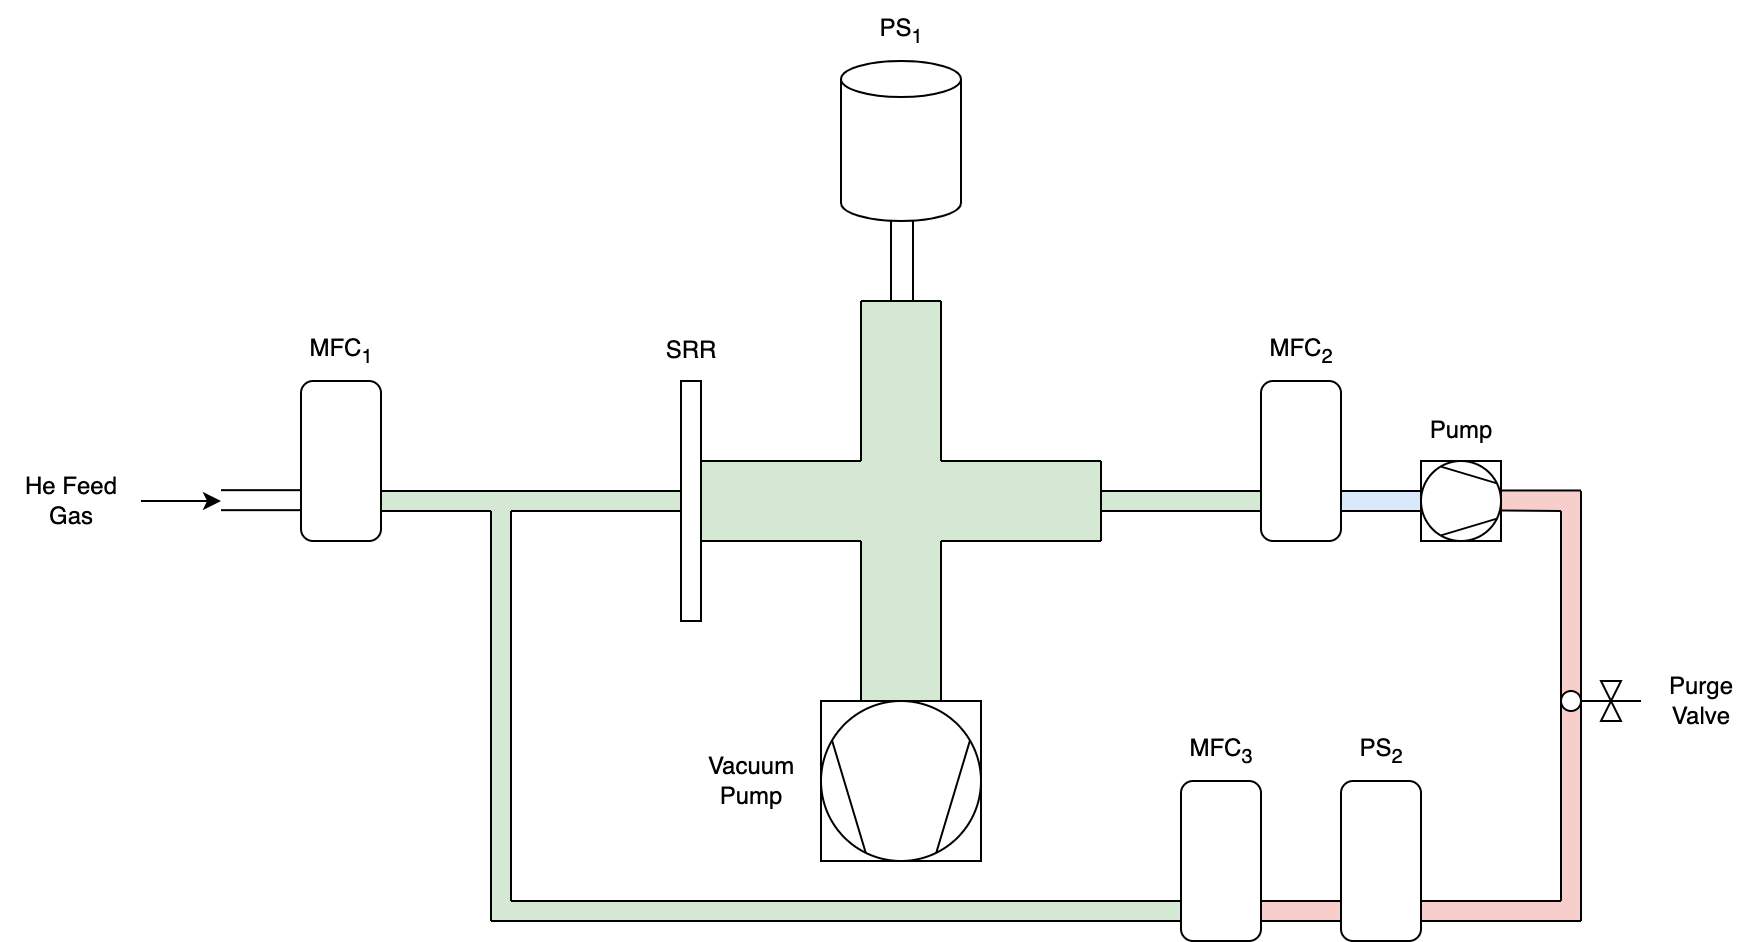
\includegraphics[width=\linewidth]{chapter_5/figures/He_control_system.png}
	\caption{Schematic of control system with helium feed gas.}
	\label{fig:He_control_system}
\end{figure}

In the aforementioned design, there are three distinct pressurised regions. The first, highlighted in green, is the region where the SRR is located, thus shall be kept at atmospheric pressure. As such a pressure sensor is required to allow the pressure in this region to be controlled. The next region, shown in blue, is just before the inlet to the pump and would be at a much lower pressure, typically close to a vacuum. The final region, noted in red, is before the steady state mass flow controller; to allow a gas to flow through, this region needs to be pressurised slightly above atmospheric pressures. Since this third region is kept above atmospheric pressure, and it is kept on the outlet side of the pump, safety measures are imperative to prevent cases where the pressure continues to build up to dangerous levels. As such, another pressure sensor is required here to notify the controller if the pressure in this region exceeds a certain threshold and to initiate a software abort. Additionally, a mechanical pressure relief valve would be wise in the case that the software abort fails for any reason. 

The equipment details used in figure \ref{fig:He_control_system} has been listed in table \ref{table:equipment_used}. One point to note is the use of a pressure controller in lieu of the second pressure sensor was due to the fact that only one capacitive pressure sensor available for the project. As such, the pressure controller was set to be normally open and was only used to sample the pressure. It was also calibrated to the capacitive pressure sensor and showed minimal error  through the range of pressures used. The mass flow controllers were calibrated from factory, as such the only change made to the devices were to the gas correction factors. 

\begin{table}[]
\centering
\caption{Name and description of equipment used for recirculation of helium only.}
\begin{tabular}{lll}
Code & Type                & Description                                            \\
\hline
MFC$_1$    & MKS GE50A, 200 sccm & Mass flow controller for (fresh) feed gas              \\
MFC$_2$    & MKS GE50A, 200 sccm & Mass flow controller for pump inlet                    \\
MFC$_3$    & MKS GE50A, 50 sccm  & Mass flow controller for (recycled) feed gas           \\
PS$_1$     & MKS 623H, 1000 Torr & \begin{tabular}[c]{@{}l@{}}Capacitance manometers for pressure in \\ primary chamber\end{tabular} \\
PS$_2$     & MKS 640B, 1000 Torr & Pressure controller for secondary chamber             
\end{tabular}
\label{table:equipment_used}
\end{table}

To design this controller, all modelling was done using MATLAB Simulink, however the implementation of the controller in code was done in Python with the use of \textit{simple-pid}, an open sourced PID controller library. A simple GUI was also designed in Python using \text{customtkinter}, and open sourced UI-library based on Tkinter, to allow information regarding the controller to be brought up in real time. Communication with the sensors and actuators were achieved via serial, as stated in the previous subchapter. The implementation of the controller can be found in the accompanying GitHub repository for this report.

\begin{figure}[h!]
    \centering
    \begin{subfigure}{0.7\linewidth}
        \centering
        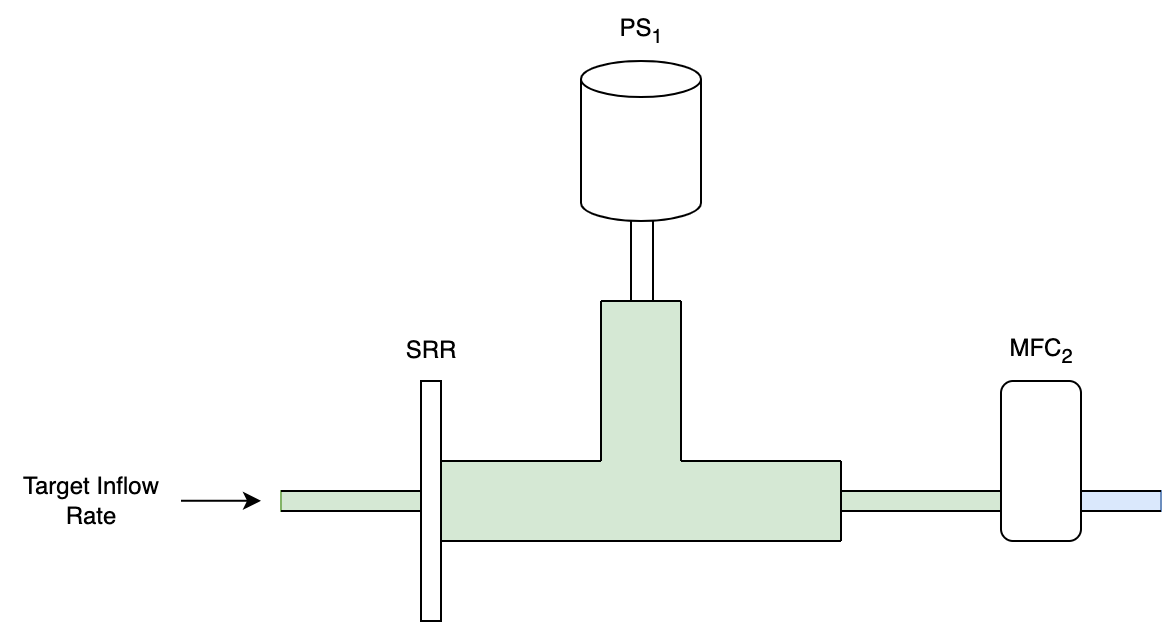
\includegraphics[width=\linewidth]{chapter_5/figures/He_chamber_pressure_controller.png}
        \caption{}
%        \label{fig:}
    \end{subfigure}
    \hfill
    \begin{subfigure}{0.7\linewidth}
        \centering
        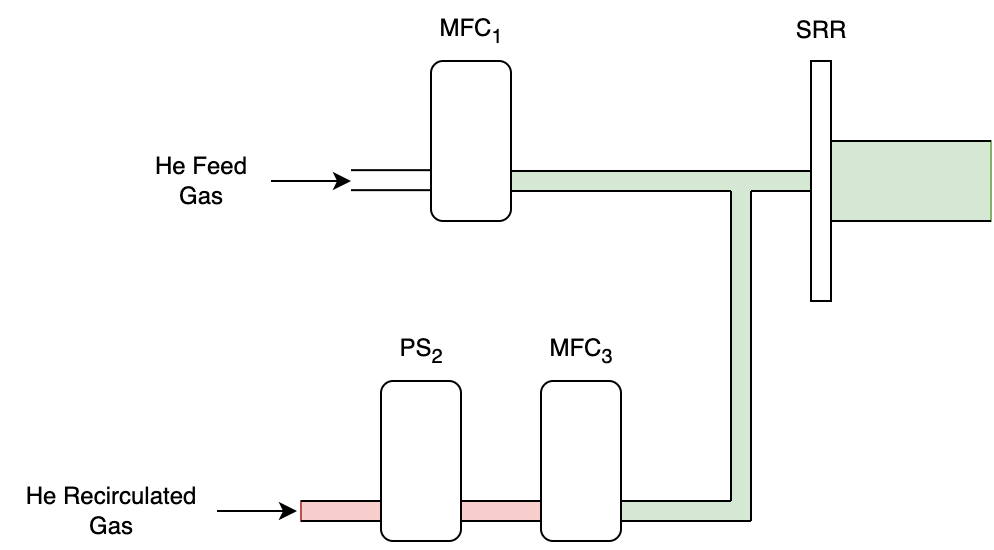
\includegraphics[width=\linewidth]{chapter_5/figures/He_target_flow_rate_controller.png}
        \caption{}
%        \label{fig:image12}
    \end{subfigure}
    \caption{Splitting control system into chamber pressure control (a) and target flow rate control (b).}
    \label{fig:He_controller_split}
\end{figure}

The control system for a helium only setup can be broken down into two stages. First, there is the depressurising of the system to take it as close to a vacuum as possible. The goal was to remove the residual gas from the system and any gas that has leaked in from the atmosphere which can affect the plasma. This process was primarily done manually as the vacuum pump did not have remote functionality. In the depressurising stage of the controller, all the mass flow controllers bar the one controlling the feed gas (MFC$_1$) were set to their maximum rated flow rate. Once this happened, the vacuum pump can be manually run until the pressure sensors read  zero Torr. 

In the second stage, the helium feed gas can be introduced into system and the controller would recirculate the gas. For this stage, it would be useful the split the setup in figure \ref{fig:He_control_system} into two disparate control designs. One of this designs is to control the pressure in the chamber housing the SRR, while the other controls the net flow rate through the SRR. These are illustrated in figure \ref{fig:He_controller_split}.


\subsection{Pressure in the SRR chamber}
\label{subsec:pressure_in_srr_chamber}

The pressure in the main chamber with the SRR was controlled by only using MFC$_2$, which controls the outflow of gas from the chamber. As the flow rate into the chamber (through the SRR) was controlled separately, it can be assumed that the flow rate into the chamber is fixed to a particular target; this can be called $Q_{t}$. Since the mass flow controllers determine the amount of gas let in and out of the chamber, its pressure can be modelled by the ideal gas law. This is possible because MFC$_2$ is located before the recirculation pump, which means that pumping speed (which is dependant on the pressure on the inlet) plays no role. 

The ideal gas law is:
\begin{equation}
    P = \frac{nRT}{V}
\end{equation} 

The pressure ($P$) is a function of the number of moles of gas ($n$), its temperature ($T$), and the volume of the main chamber ($V$). $R$ is simply the gas constant. Both the temperature of the chamber and its volume are constant. Though there is heat generated from the plasma, its area of affect is much smaller compare to the size of the chamber, thus it is effectively constant. Hence the only variable is $n$. Taking the partial derivative of the pressure with respect to the number of moles gives: 

\begin{equation}
    \left( \frac{\partial P}{\partial n} \right)_{T,V}= \frac{RT}{V} \frac{\partial n}{\partial t}
\end{equation}

The number of moles can be derived as a product of the net flow rate ($Q_{net}$) and time, which is expressed as: 
\begin{equation}
    n = Q_{net} t
\end{equation}

And its derivative with respect to time is:
\begin{equation}
    \frac{\partial n}{\partial t} = Q_{net}
\end{equation}

Thus, the rate of change of pressure in the system is governed by:
\begin{equation}
    \left( \frac{\partial P}{\partial t} \right)_{T,V}  = \frac{RT}{V} Q_{net}
    \label{eq:rate_of_change_of_pressure}
\end{equation}

While this is an analytical solution, the issue is that the volume of the chamber is unknown. While it is possible to get an approximate volume by taking measurements of the chamber and hose lengths, it would be simpler to determine numerically. However rather than just determining the volume, the constant $\frac{RT}{V}$ can be determined instead. To achieve this, the change of pressure with respect to time was measured across several net flow rates from 10 sccm to 50 sccm. This is shown in figure \ref{fig:rate_of_change_of_presure}.

\begin{figure}[h!]
	\centering
	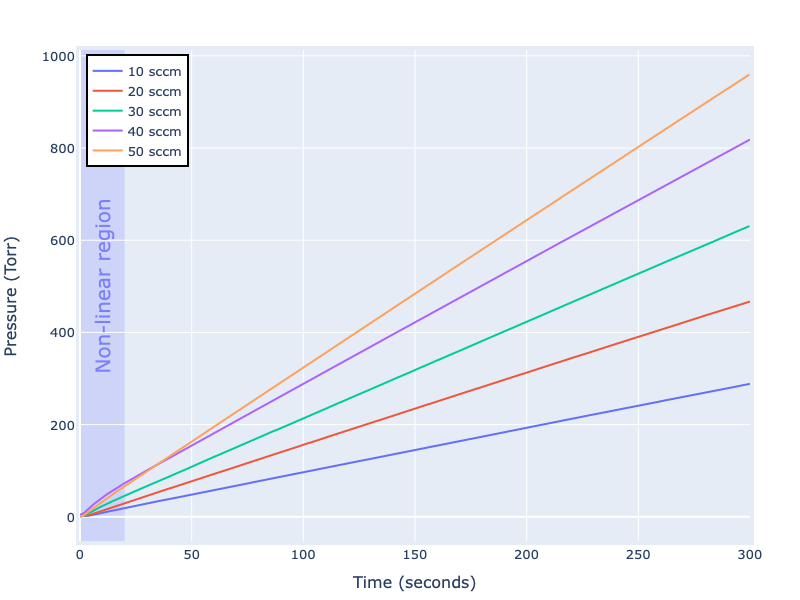
\includegraphics[width=\linewidth]{chapter_5/figures/rate_of_change_of_pressure.png}
	\caption{Rate of change of pressure in main chamber for flow rates between 10-50 sccm.}
	\label{fig:rate_of_change_of_presure}
\end{figure}

The gradient of the slope express the right hand side of equation \ref{eq:rate_of_change_of_pressure}. While not visible from the figure, there are some non-linearity in the beginning of the slope when the pressure increases from zero Torr. This is primarily due to the transients from the mass flow controllers turning on and typically settle after around 15-20 seconds. The average slope across all the flow rates tested from between 20-300 seconds are shown in table \ref{table:rate_of_change_of_pressure}.

\begin{table}[]
\centering
\begin{tabular}{cc}
Flow rate (sccm) & Average rate of change of pressure (Torr/s) \\
10               & 0.960 $\pm$ 0.237                   \\
20               & 1.558 $\pm$ 0.330                   \\
30               & 2.089 $\pm$ 0.181                   \\
40               & 2.655 $\pm$ 0.116                   \\
50               & 3.189 $\pm$ 0.129                             
\end{tabular}
\caption{Average rate of change of pressure measured for flow rates between 10-50 sccm.}
\label{table:rate_of_change_of_pressure}
\end{table}

\begin{figure}[h!]
	\centering
	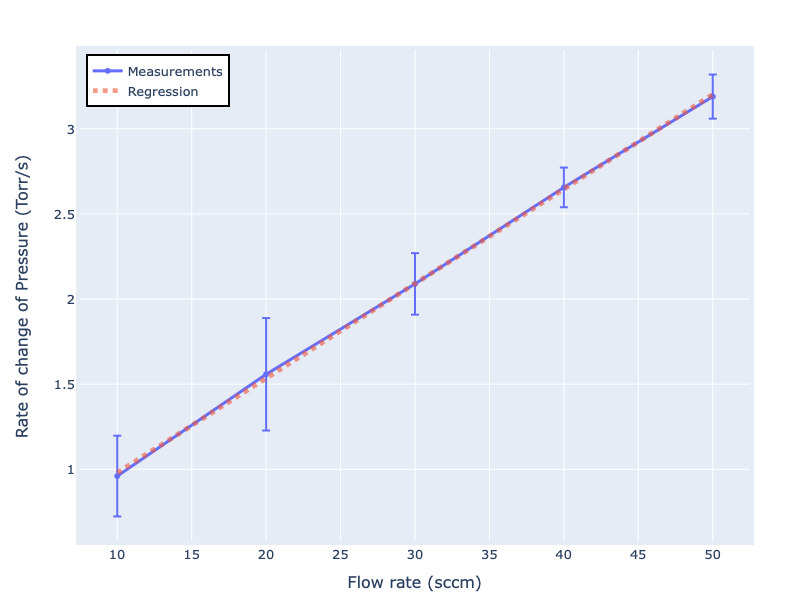
\includegraphics[width=\linewidth]{chapter_5/figures/gradient_rate_of_change_of_pressure.png}
	\caption{Relationship between rate of change of pressure and flow rate.}
	\label{fig:gradient_rate_of_change_of_pressure}
\end{figure}

When graphing the data from table \ref{table:rate_of_change_of_pressure}, a linear relationship is observed; though not a perfect one. This is shown in figure \ref{fig:gradient_rate_of_change_of_pressure}. A line of best fit can be taken in order to determine the value of the constant $\frac{RT}{V}$, which would be the slope of the graph. The gradient was determined to be 0.055 Torr min cm$_{STP}^{-3}$. Therefore the solution for the rate of change of pressure is:
\begin{equation}
    \frac{dP}{dt} = 0.055 Q_{net}
\end{equation}

This new equation can be used as the transfer function to represent the plant for the control system. Applying a Laplace transform gives the plant transfer function:

\begin{equation}
    P(s) = \frac{0.558}{s} Q_{net}(s)
    \label{eq:transfer_function}
\end{equation}

With the plant characterised, the control system can be built. A typical control system has three parts: the sensors, the actuators, and the control algorithm itself (henceforth simply referred to as the controller). The basic control system model for the plant is shown in figure \ref{fig:control_system}. The term $P_{set}$ corresponds to the set point pressure, $Q_d$ to the drive flow rate suggested by the controller, and $P_m$ is the measured pressure. In the case without the sensor and actuator blocks, $Q_d$ and $P_m$ correspond to $Q_{net}$ and $P$ respectively.  The rational for incorporating the sensors and actuators into the model is to take into account factors that produce errors such noise or bias. However, at first it would be best to simply design a controller assuming ideal circumstances. 

\begin{figure}[h!]
	\centering
	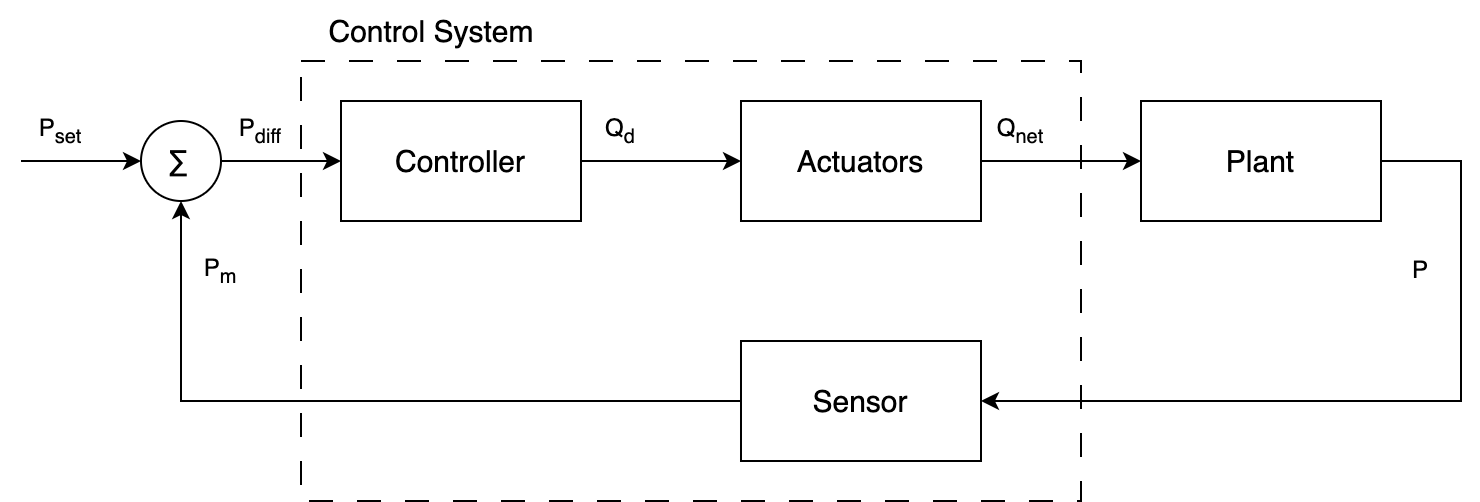
\includegraphics[width=\linewidth]{chapter_5/figures/control_system.png}
	\caption{Basic schematic of control system.}
	\label{fig:control_system}
\end{figure}
 
To start, the proportional controller modelled in figure \ref{fig:p_controller} was used. In essence, this controller adjusts the output based on the error between the set point and measured pressure value (called the process variable). Therefore as the error increases, the correction applied also increases. The correction can be adjusted using a proportional term called $K_p$, which is simple a fixed gain. The value of $K_p = 5$ was chosen arbitrarily. To evaluate the controller, three test cases were devised. These include:

\begin{itemize}
    \item \textbf{Test case 1} - Bringing the chamber up to 760 Torr from a vacuum, which would simulate the case of flushing the system and re-pressurising it.
    \item \textbf{Test case 2} - Brining the chamber up to 760 Torr from 720 Torr (approximately 95\% of the set point), which would simulate a steady state case where there was a small drop in pressure in the system.
    \item \textbf{Test case 3} - Brining the chamber down to 760 Torr from 800 Torr (approximately 105\% of the set point), which would simulate a steady state case where there was a build up of pressure in the system.
\end{itemize}

\begin{figure}[h!]
	\centering
	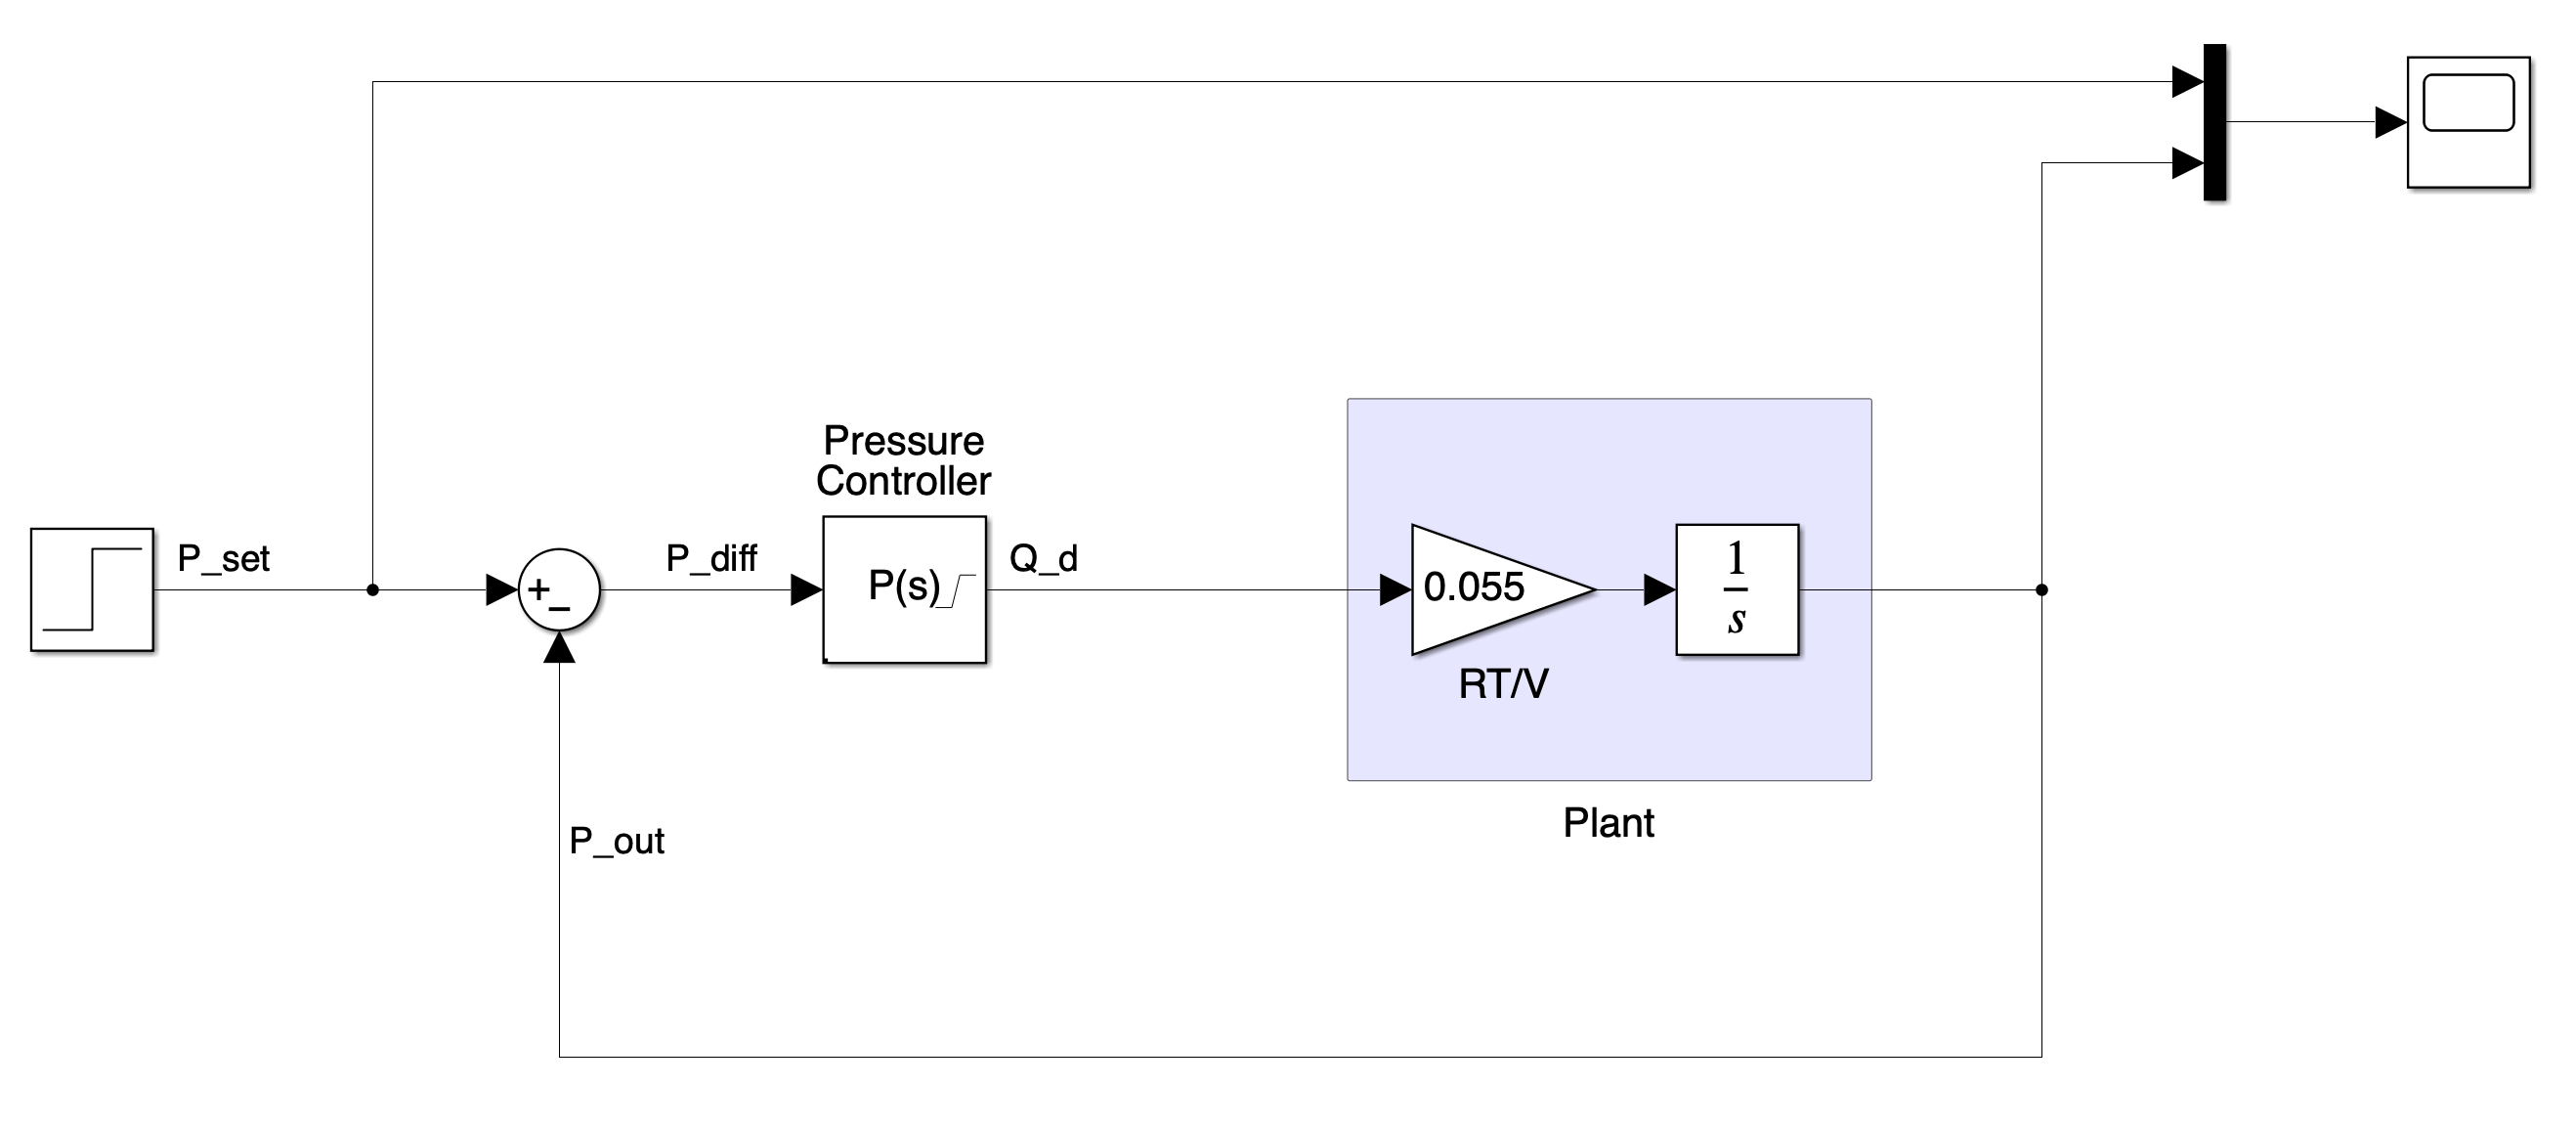
\includegraphics[width=\linewidth]{chapter_5/figures/p_controller.png}
	\caption{Illustration of control system.}
	\label{fig:p_controller}
\end{figure}

The results for the proportional controller can be seen in figures \ref{fig:kp_results_no_actuators} (seen as P - No saturation). Note, for the purposes of quantifying the results, the term settling time is defined as the time taken for the controller to settle to within 0.1\% of the set value; which is approximately $\pm1$ Torr for a set value at atmospheric pressure. 

\begin{figure}[h!]
    \centering
    \begin{subfigure}{0.8\linewidth}
        \centering
        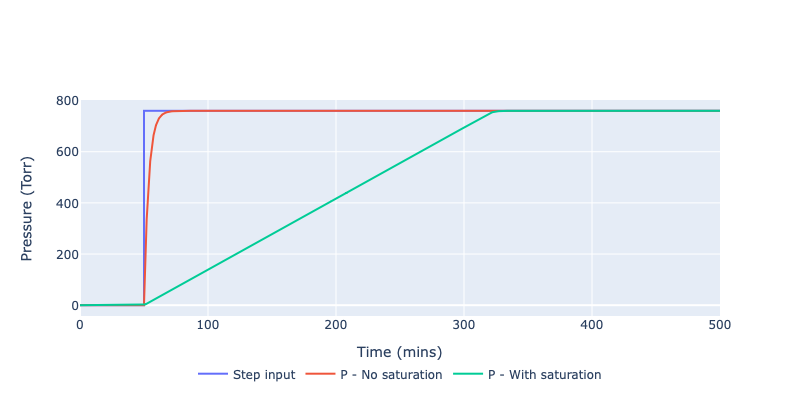
\includegraphics[width=\linewidth]{chapter_5/figures/test_1_kp.png}
        \caption{}
%        \label{fig:}
    \end{subfigure}
%    \hfill
    \begin{subfigure}{0.8\linewidth}
        \centering
        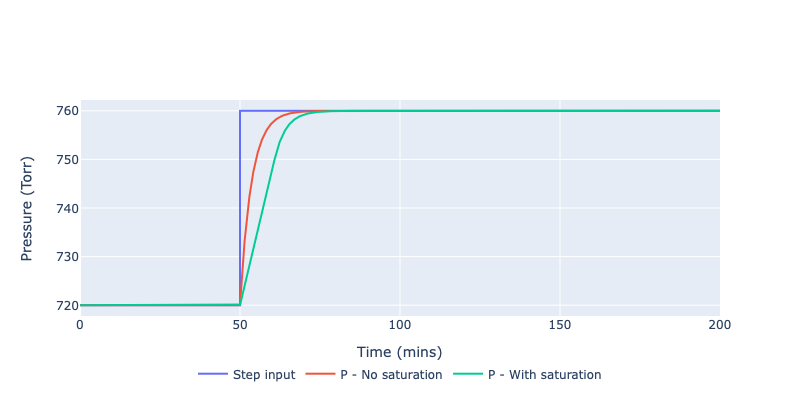
\includegraphics[width=\linewidth]{chapter_5/figures/test_2_kp.png}
        \caption{}
%        \label{fig:image12}
    \end{subfigure}
   
    \bigskip
    \begin{subfigure}{0.8\linewidth}
        \centering
        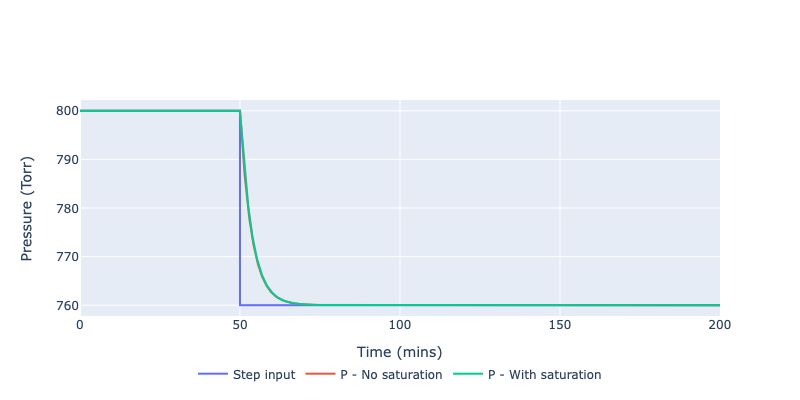
\includegraphics[width=\linewidth]{chapter_5/figures/test_3_kp.png}
        \caption{}
%        \label{fig:image3}
    \end{subfigure}
    \caption{Evaluation of proportional controller for test cases 1 (a), 2 (b), and 3 (c).}
    \label{fig:kp_results_no_actuators}
\end{figure}

The basic controller seems to perform well with no overshoot and a settling time of 19 seconds for the first test case, and 8.5 seconds for the second and third test case. However, such performance is unobtainable in the real world as the drive flow rate is beyond the capabilities of the mass flow controllers used. When the drive flow rate is saturated within the constraints of the mass flow controllers used, the settling times increase to 273.5 seconds for the first test case, 14.3 seconds for the second, and 8.6 seconds for third. The saturation values chosen were between a maximum of 50 sccm to a minimum of -150 sccm. This is because the maximum drive flow rate is achieved when the outlet mass flow controller is set to zero, whilst the minimum flow rate is achieved when the outlet mass flow controller is set to its maximum value of 200 sccm. The results with the output saturation of the controller are also shown on figure \ref{fig:kp_results_no_actuators} (seen as P - With saturation). Note that the times are noticeably longer for both test 1 and 2, however test 3 only shows a marginal decrease in settling time. This is because of the asymmetry of the drive flow rate, where the controller can more quickly get rid of gas in the chamber than it can fill it up. 

Now that a controller was designed for the ideal control system, the sensor and actuator blocks can be reintroduced. Starting with the actuators, the data sheet states that the mass flow controllers have a typical accuracy of ``$\pm$1\% of set point for 20 to 100\% Full Scale, $\pm$0.2\% of Full Scale for 2 to 20\% Full Scale" \cite{mks_ge50}. Based on the equipment used (the details of which can be found in table \ref{table:equipment_used}), the systematic error for the mass flow controllers would be $\pm$2 sccm. As for the sensors, the data sheet states that the capacitive pressure sensor used has accuracy of ``$\pm$0.25\% of reading" \cite{mks_623h} for the pressure sensor; and ``$\pm$0.5\% of reading" for the pressure controller \cite{mks_640b}. Assuming the worst case, this would mean that the systematic error in the sensor would be $\pm$3.8 Torr. Errors caused by environmental affects would be difficult to model, thus are ignored in the model.

The updated Simulink model can be seen in figure \ref{fig:pi_controller}, where these errors were modelled as constants. The terms $Q_{in}$ and $Q_{out}$ are the input and output flow rates governed by MFC$_1$ and MFC$_2$. Note that the controller is designed to control the net flow rate in or out of the chamber, hence the value for $Q_{out}$ was determined by taking the difference between $Q_{in}$ and $Q_{d}$. As for the value of the error constants, these were set to take the maximum possible errors specified in the previous paragraph.

\begin{figure}[h!]
	\centering
	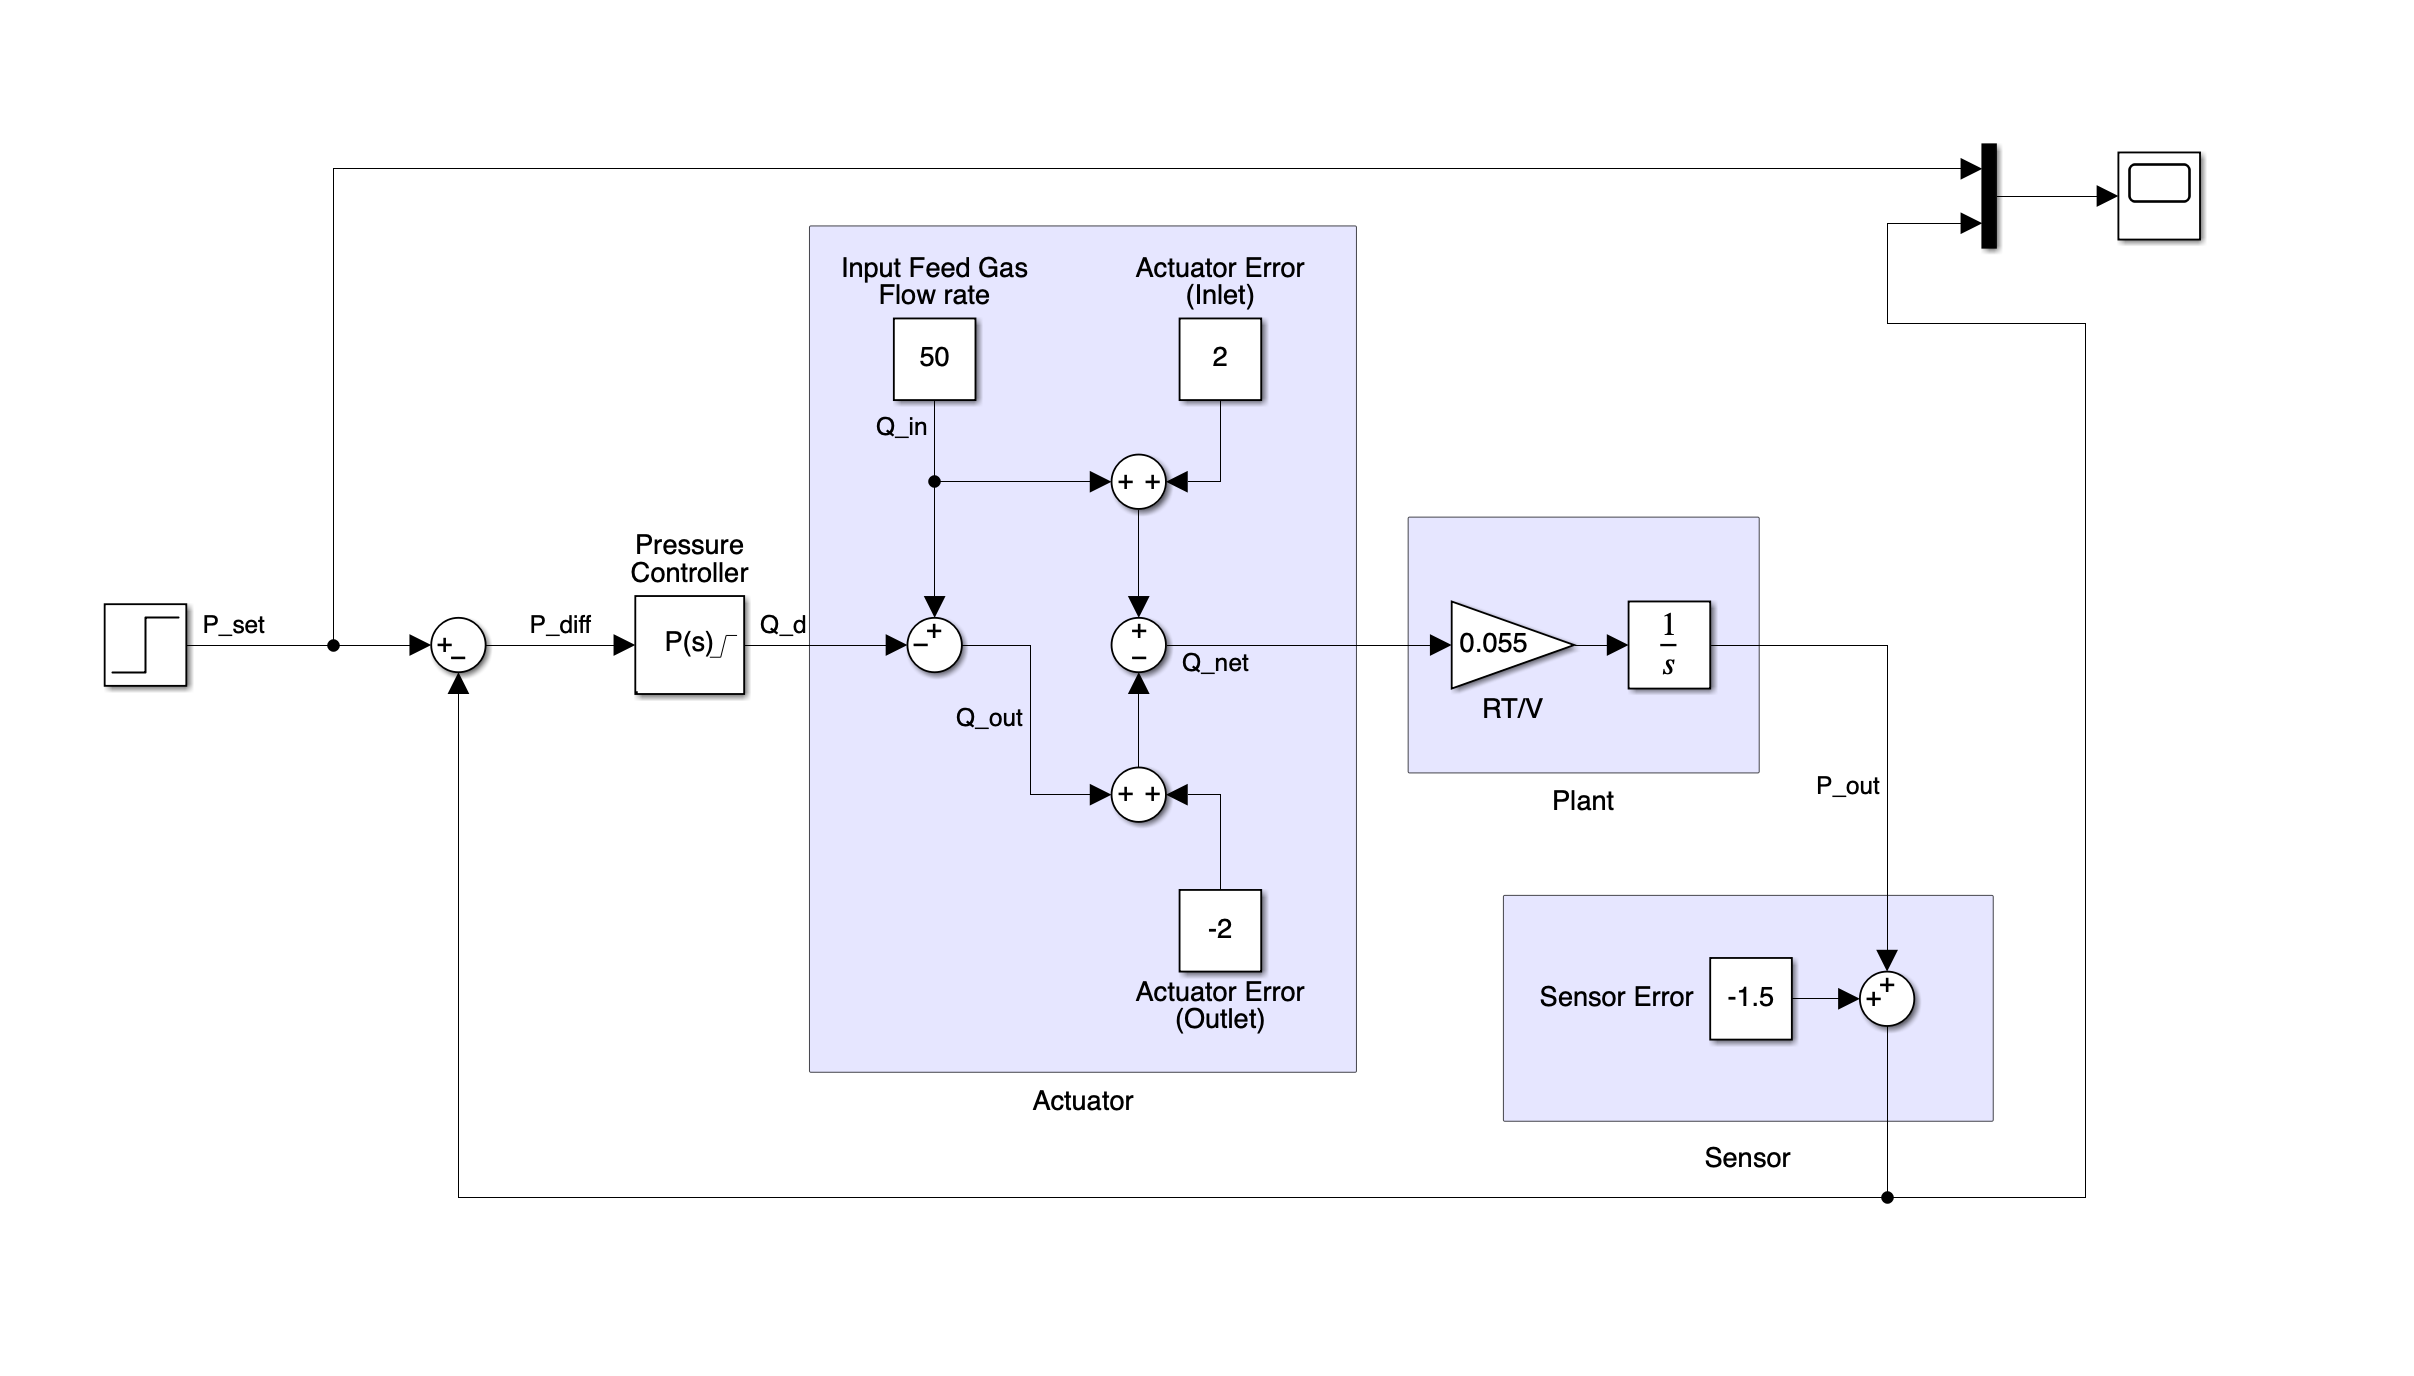
\includegraphics[width=\linewidth]{chapter_5/figures/pi_controller.png}
	\caption{Illustration of control system.}
	\label{fig:pi_controller}
\end{figure}

Introducing these constant error terms into the model caused a steady state offset to be observed in all three test cases. The magnitude of the offset was the same for each test case, meaning they are independent of the pressure. An intuitive explanation for this is that the controller is attempting to send the correct signal to the plant, but the error from actuator or sensor cancels out the drive signal, hence no change occurs in the plant. A visualisation of these offsets can be seen in figure \ref{fig:sensor_actuator_error}, which highlights the effect that varying the systematic error has on the offset. The impact of the errors from the actuators and sensors were compared separately.

\begin{figure}[h!]
	\centering
	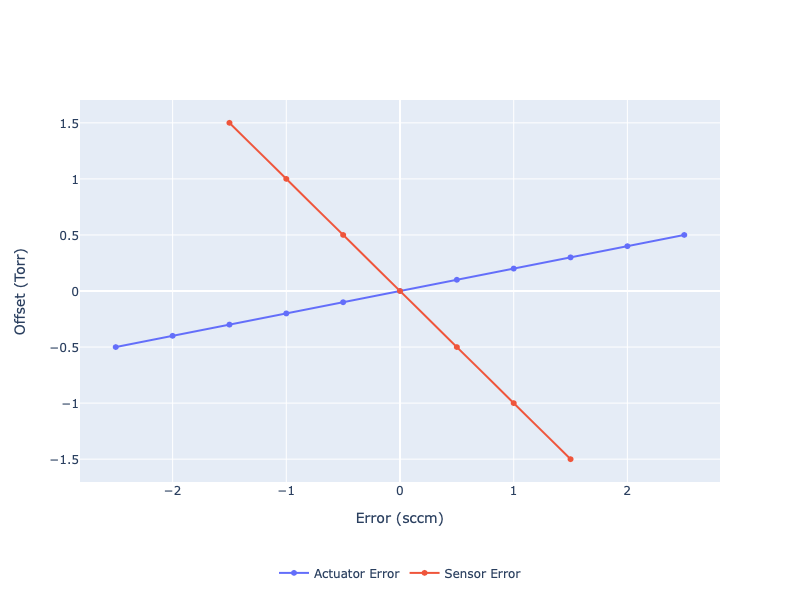
\includegraphics[width=\linewidth]{chapter_5/figures/sensor_actuator_error.png}
	\caption{Comparison of offset introduced by the actuator and sensor error.}
	\label{fig:sensor_actuator_error}
\end{figure}

In order to get rid of this, the introduction of an integrator component to the controller is needed. The integrator adjusts the output of the controller based on the accumulated error over time. As the duration or magnitude of an error increases, so does the correction factor. Thus, the integral term compensates for any steady state error in the system. One common  trade off with the integrator component is called overshoot, where the lag introduced by the integrator causes the controller to not respond fast enough, This results in the controller overshooting the set point. To control this, an integrator term, $K_i$, can be introduced. 


Another limitation with using an integrator component called integral windup. This is especially apparent in a system where the actuators have an upper and lower limit to the amount of drive signal it can produce. Windup occurs due to a large accumulation of error between the set point and process variable, then when the sign of the error is flipped, time is required to unwind the accumulated error. The result is an excessive overshoot, which cannot be eliminated using $K_i$. 


An illustration of can be seen in figure \ref{fig:windup}, shown using test case 1. With $K_i=0.01$, resulted in an overshoot to 940 Torr (nearly 24\% over the set point pressure). The windup is simply the accumulation of the error, shown as the area between the the step input and the response in orange. Then as the the response overshoots, the integral error drops until it reaches the maximum point. Finally, the error is unwound as shown in the graph as the green area; the error is fully unwound when the green area is equal to the orange area. In order to address this problem, a process called clamping is used. This is achieved by preventing the integrator component from accumulating error by limiting its value within a certain upper and lower bound. 

\begin{figure}[h!]
	\centering
	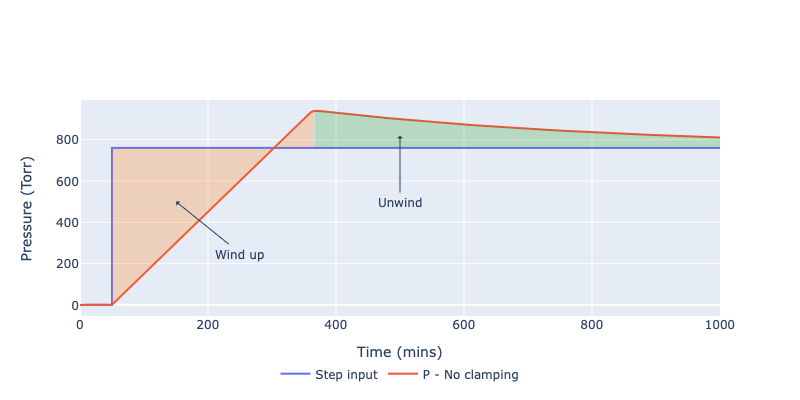
\includegraphics[width=\linewidth]{chapter_5/figures/windup.png}
	\caption{Illustration of integral windup for PI controller ($K_p = 5$, $K_i = 0.01$).}
	\label{fig:windup}
\end{figure}

Thus, the resulting controller (with a proportional and integrator component) is known an a PI controller. The final proportional and integral terms selected were $K_p = 5$ and $K_i = 1$, which were determined heuristically. The goal when tuning the controller was to balance settling time and overshoot, whilst avoiding oscillations. The rational for avoiding oscillation was to minimise any disturbances to the plasma that could potentially cause it to die out. A comparison of several $K_i$ values are shown in figure \ref{fig:ki_results}. Note that the impact of varying the $K_i$ values in test case 1 were minimal in terms of overshoot, with the only observable changes being the settling time. 

\begin{figure}[h!]
    \centering
    \begin{subfigure}{0.8\linewidth}
        \centering
        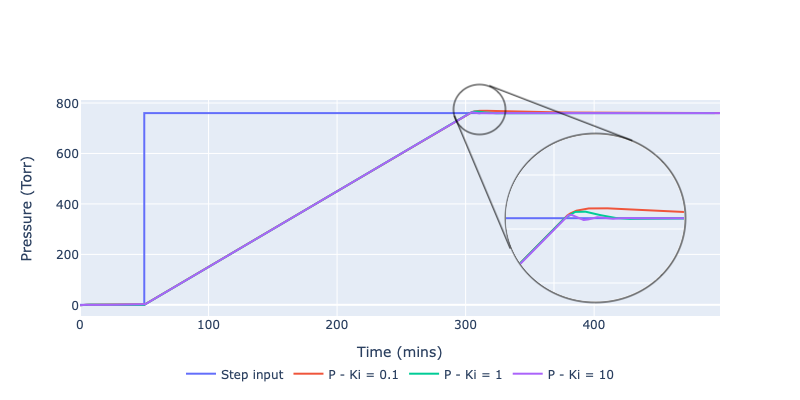
\includegraphics[width=\linewidth]{chapter_5/figures/test_1_ki.png}
        \caption{}
%        \label{fig:}
    \end{subfigure}
%    \hfill
    \begin{subfigure}{0.8\linewidth}
        \centering
        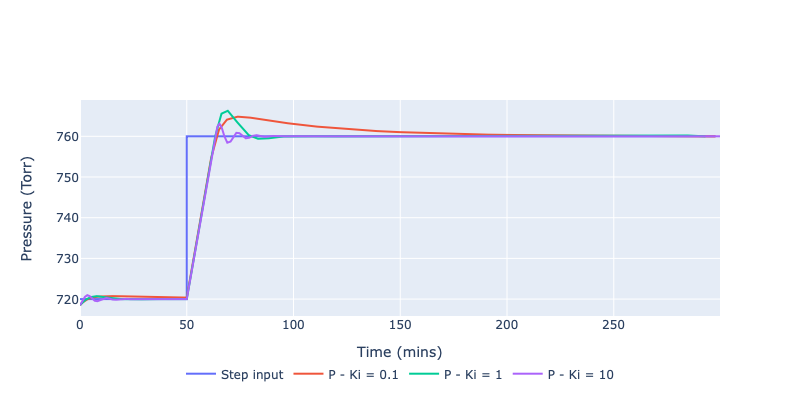
\includegraphics[width=\linewidth]{chapter_5/figures/test_2_ki.png}
        \caption{}
%        \label{fig:image12}
    \end{subfigure}
   
    \bigskip
    \begin{subfigure}{0.8\linewidth}
        \centering
        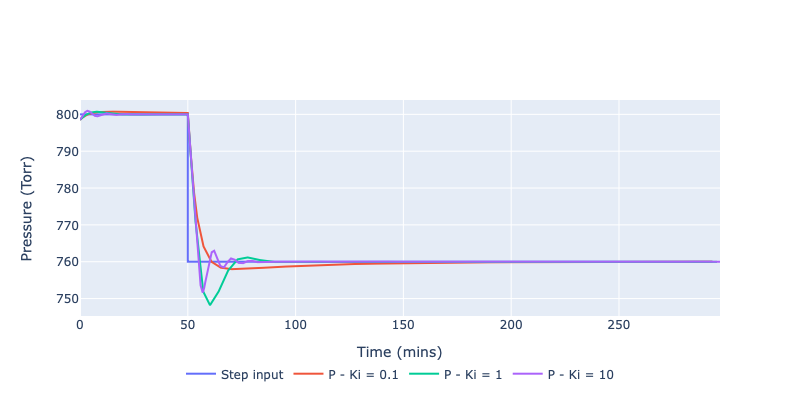
\includegraphics[width=\linewidth]{chapter_5/figures/test_3_ki.png}
        \caption{}
%        \label{fig:image3}
    \end{subfigure}
    \caption{Evaluation of PI controller for test cases 1 (a), 2 (b), and 3 (c).}
    \label{fig:ki_results}
\end{figure}

When modelling, the time step selected was 1 second. This specific value was chosen to allow sufficient time to read data from the sensors and send commands to the actuators. Additional buffer time was included for cases when the sensors or actuators fail to acknowledge the commands sent to it.

The PI controller in Simulink, was translated into Python code. The controller was expressed in the following form:
\begin{equation}
    Q_d(t) = K_p P_e(t) + K_i \int_{0}^{t} P_e(t) dt
    \label{eq:pi_controller}
\end{equation} 

The performance of the real controller was evaluated using the first test case, with the results shown in figure \ref{fig:pi_performance}. When compared the the model, the real controller performed worse when it came to the overshoot but slightly better in terms of settling time. The overshoot value was nearly doubled from 5.8  to 10.6 Torr. However, this overshoot is just over 1\% of the of the set point, which was thought be to an acceptable performance. The settling time of the real controller 261 seconds, about 6 seconds faster than the model but is within the margin of error. The discrepancy observed at the start of the step input are the same non-linearities seen in \ref{fig:rate_of_change_of_presure}.

\begin{figure}[h!]
	\centering
	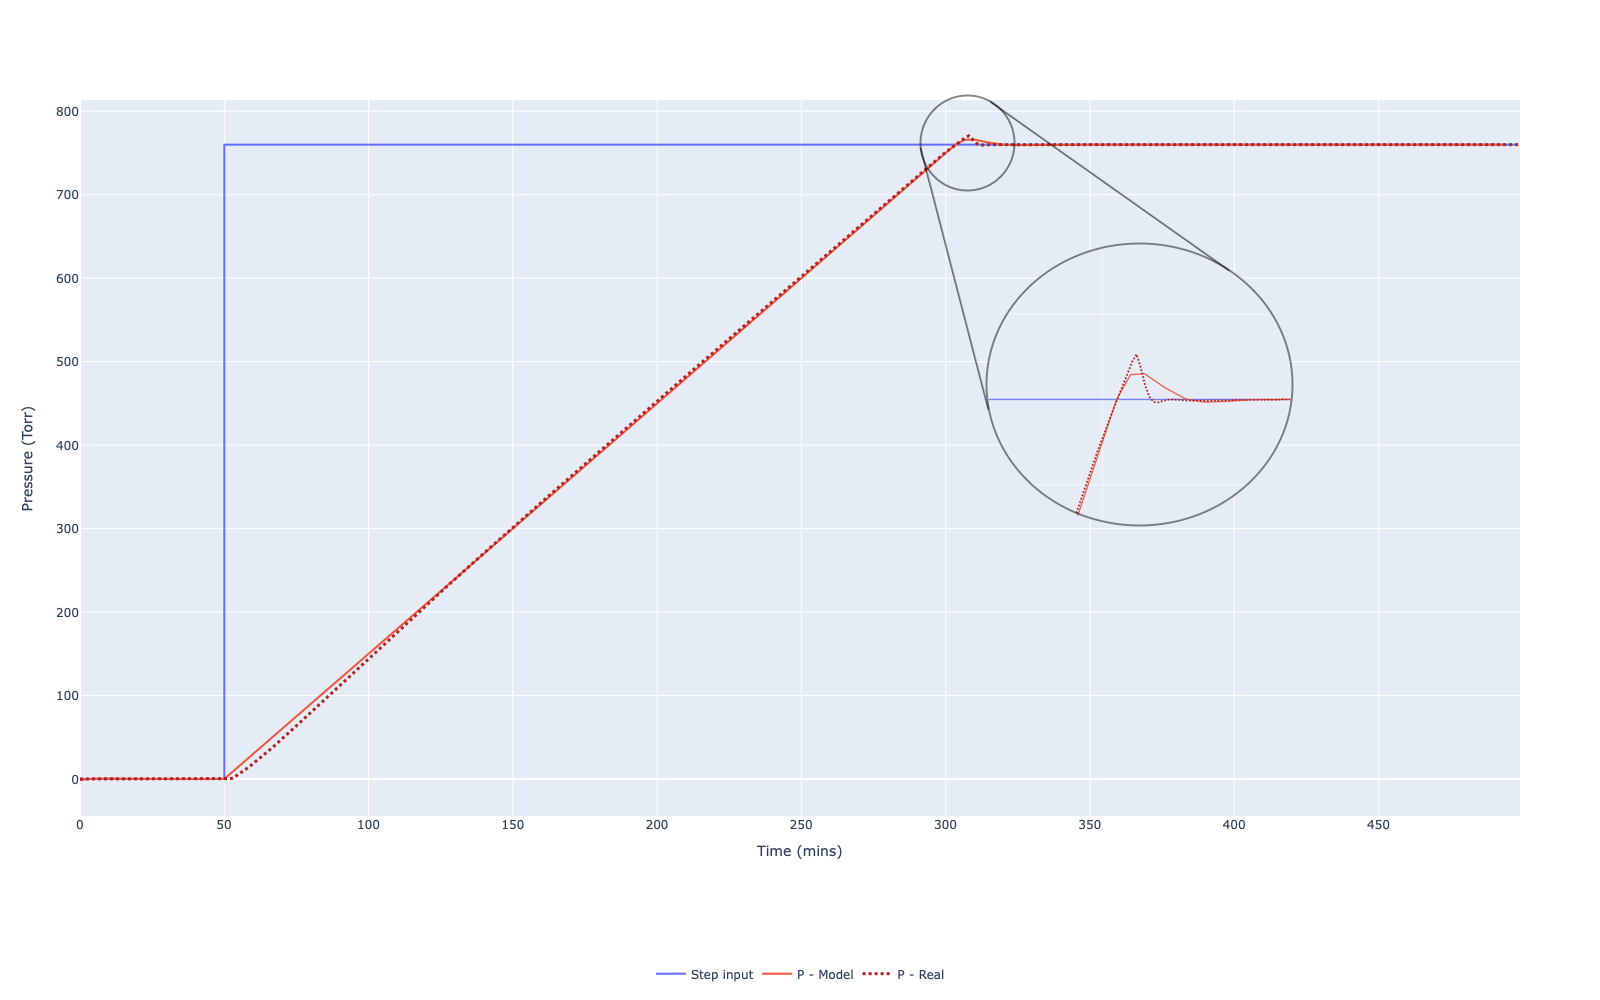
\includegraphics[width=\linewidth]{chapter_5/figures/real_pi_vs_model.png}
	\caption{Comparison between the performance of the modelled and real PI controllers.}
	\label{fig:pi_performance}
\end{figure}



\subsection{Flow rate to the SRR}

With the PI controller designed, the second stage of the control system was to regulate the flow rate to the SRR. After depressurising the system, it needs to be first refilled with Helium feed gas from the tank, henceforth referred to as \textit{fresh gas}. Then as the main chamber and secondary chamber is pressurised, the dependance on fresh gas can be reduced in favour of the recirculated Helium from the secondary chamber; simply referred to as \textit{recycled gas}. Whilst this is occurring, the net flow rate through the SRR needs to be kept constant at the target flow rate. 

The value for target flow rate is limited by the maximum flow rate of MFC$_3$ which was 50 sccm. So the first step was to determine what level of pressure difference is required between the inlet and outlet of the mass flow controller (MFC$_3$) to achieve a steady flow rate of 50 sccm. The data sheet for the mass flow controllers state that the normal operating pressure differential was ``10 to 40 psid at 10 to 5000 sccm" \cite{mks_ge50}. This equates to a pressure difference of over 500 Torr between the inlet and the outlet. However from some experimentation, it was found that the pressure difference required ranged from around 100 to 200 Torr, with the difference increasing as the outlet pressure is dropped below atmospheric pressure.

Since the outlet was at atmospheric pressures, the pressure difference of at least 100 Torr is required to to ensure that target flow rate is achieved with only using the recycled gas. Based on this, the selected pressure differential chosen was slightly higher at 150 Torr. This was simply to give a slight buffer in the case where the outlet pressure is higher than atmospheric pressure, meaning that the pressure in the secondary chamber would be 910 Torr in the steady state.

Armed with this information, a controller can be designed to regulate the target flow rate to the SRR. Rather than building a second PI controller, these two parameters (fresh gas and recycled gas) can be controlled algebraically. The simplest equation to govern this is:

\begin{equation}
    Q_f = Q_t - Q_r
    \label{eq:fresh_equation}
\end{equation}

where $Q_t$ corresponds to the target flow rate at the SRR, $Q_f$ is the flow rate of fresh gas, and $Q_r$ is the recycled flow rate.

Then based on the pressure readings from PS$_1$ and PS$_2$ the recycled flow rate can be expressed as function of pressure and the target flow rate:
\begin{equation}
    Q_r = \frac{1}{150} P_{diff} Q_t 
    \label{eq:almost_recycled_equation}
\end{equation}

where $P_{diff}$ is the pressure difference between PS$_1$ and PS$_2$. 

%Based on the previous chapter, it is known that the pressure before the orifice of the SSR is slightly higher than the pressure after. This means that the reading from PS$_1$ would be slightly inaccurate, even if the difference is small. But due to the buffer added to the target pressure differential, this issue can be ignored.

Equation \ref{eq:almost_recycled_equation} is only valid for cases where $P_{diff} \geq 0$ and $P_{diff} \leq 150$, thus a more complete expression would be:

\begin{equation}
    Q_r = 
    \begin{cases}
        0,                          & \text{if } P_{diff} < 0\\
        Q_t,                        & \text{else if } P_{diff} > 150\\
        \frac{1}{150} P_{diff} Q_t, & \text{otherwise}
    \end{cases}
    \label{eq:recycled_equation}
\end{equation}

Thus, the flow rate of fresh gas (through MFC$_1$) can be controlled using equation \ref{eq:fresh_equation} and the flow rate of recycled gas through (through MFC$_3$) can be controlled via equation \ref{eq:recycled_equation}. 



%When translating these into Python code, an additional check was performed to ensure that sum of the the two flow rates equals the target flow rate. 

\subsection{Complete control system}

As mentioned earlier, the detailed implementation of the Python code is not included here. However, the full control system algorithm is expressed in the form of a flow chart seen in figure \ref{fig:he_controller_flow_chart}. 

\begin{figure}[h!]
	\centering
	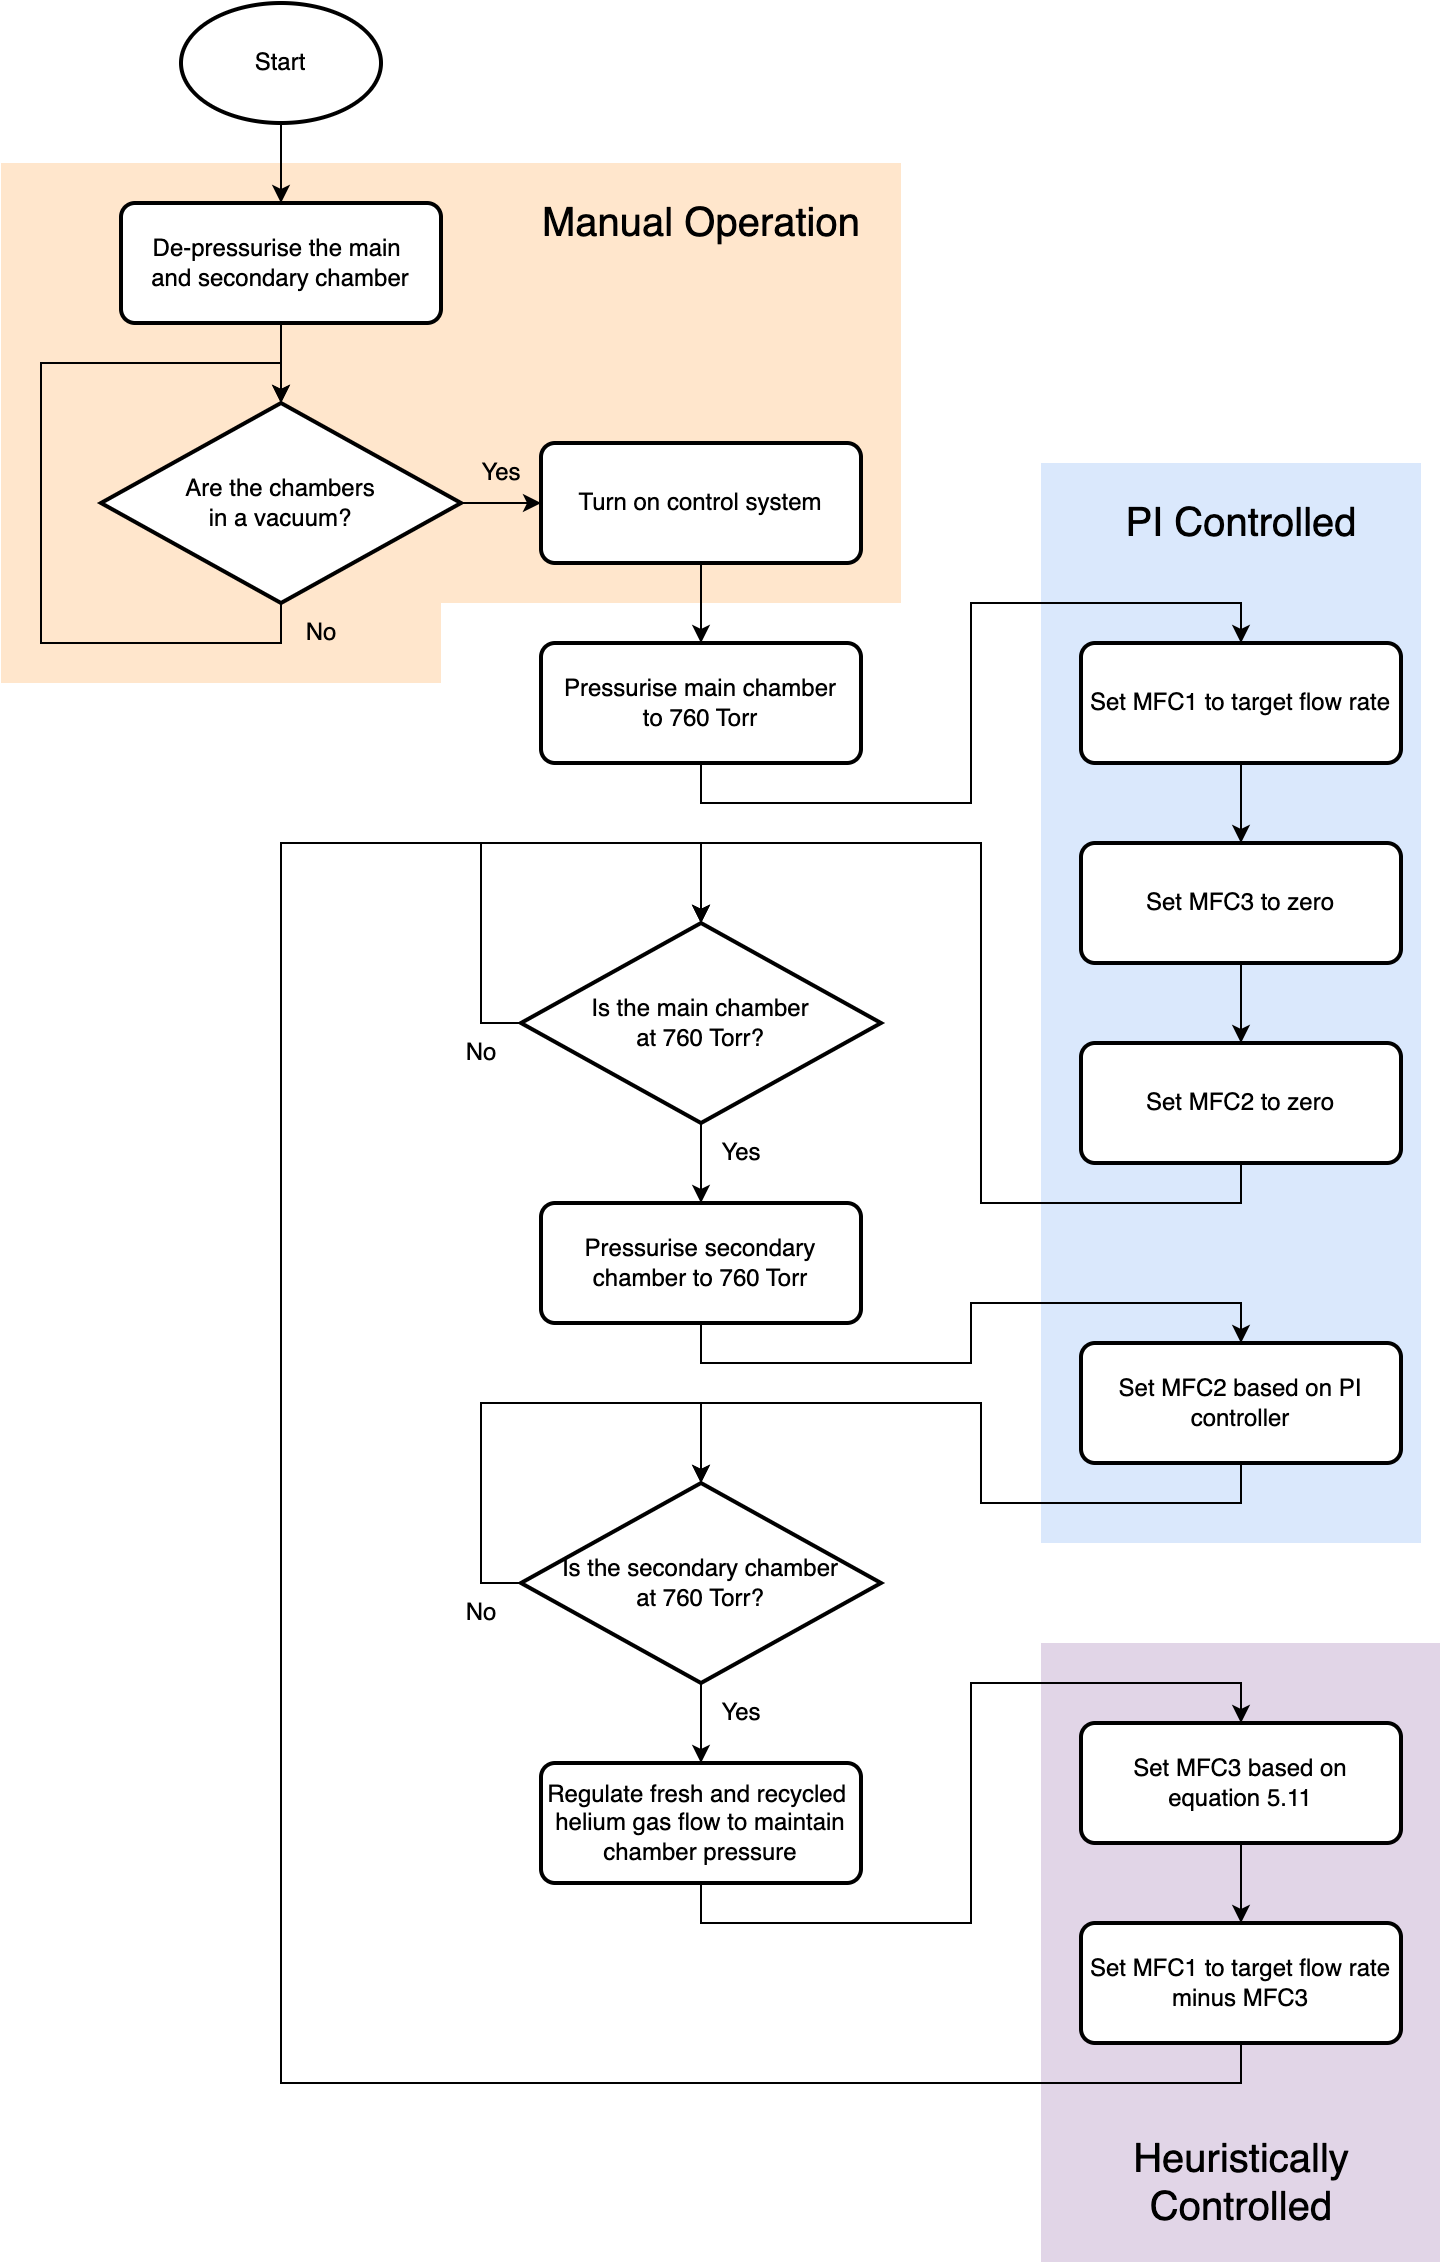
\includegraphics[width=\linewidth, height=0.9\textheight]{chapter_5/figures/He_control_flow_chart.png}
	\caption{Flow chart of Helium only recirculation control system.}
	\label{fig:he_controller_flow_chart}
\end{figure}

\pagebreak



% ---

%
%Once this process is done, the next step is to pressurise the green region (i.e. the region with the SRR). This is achieved by setting MFC$_1$ to its maximum flow rate and setting both MFC$_2$ and MFC$_3$ to zero. As the pressure in the green region approaches the target pressure, the flow rate through MFC$_2$ is increased gradually until it reaches a steady state. At this point, the flow rates of MFC$_1$ and MFC$_2$ should be the same. This leads on the the third stage of the controller, which is pressurising the red region of the setup. Here the flow rate through MFC$_2$ behaves as the inlet, and the pressure in this region also increases until a target pressure. Finally once the target pressure in the red region has been achieved, MFC$_1$ can be turned off and MFC$_3$ would be turned on (with a flow rate matching that set in MFC$_1$) to allow the Helium gas to recirculate; with MFC$_1$ only turning on when the pressure in the green region of the system drops below the minimum allowable threshold. 

\section{Control System with Helium and Carbon Dioxide}

In order to introduce CO$_2$ into the control system, a fourth  mass flow controller (MFC$_4$) was required. If the system were to be an open gas loop design, the gas composition could simply be measured as a ratio of the flow rates of CO$_2$ and Helium. Though it is a crude method, this was precisely how the concentration of CO$_2$ was determined during the characterisation experiments in the previous chapter. However in a closed gas loop design, this method of detection would not be feasible as the CO$_2$ concentration would build up over time. Instead, the gas composition would be determined using the Fourier-transform infrared spectroscopy (FTIR) spectrometer, using the correlation data of CO$_2$ concentration with absorbance (seen in $\S$ \ref{subsec:helium_and_co2}). 

These two additional components can be seen in the updated schematic drawing seen in figure \ref{fig:He_CO2_control_system}. There are several important points to note about the positioning of these components in relation to each other in the setup. 

\begin{figure}[h!]
	\centering
	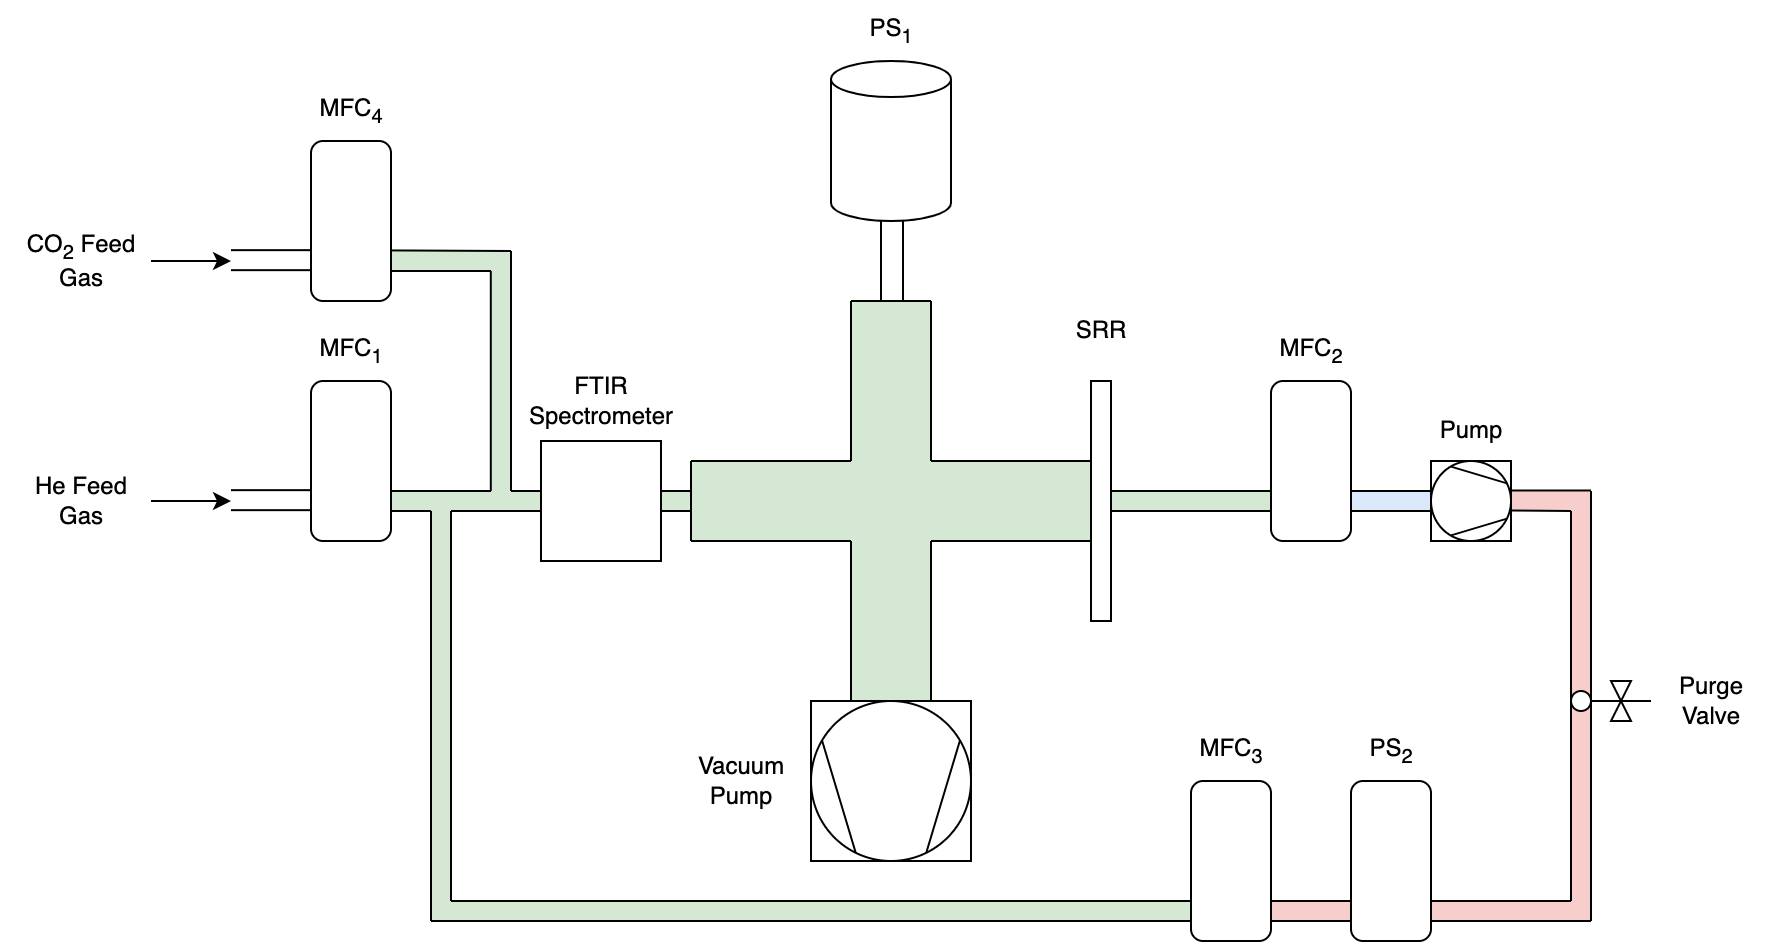
\includegraphics[width=\linewidth]{chapter_5/figures/He_CO2_control_system.png}
	\caption{Schematic of control system with helium feed gas and carbon dioxide.}
	\label{fig:He_CO2_control_system}
\end{figure}


Firstly is with regards to the position of the FTIR spectrometer located before the SRR. Initially, the idea was to position the spectrometer after the SRR in order to measure the gas composition immediately after the plasma, which would be useful in the later experiments involving the trans-stilbene liquid. However from experimentation, it was found that positioning the spectrometer behind the SRR there would cause a relatively large lag time between when the CO$_2$ was first introduced into the system to when the it detected by the spectrometer. This has to do with the fact that the volume of the main chamber is several orders of magnitude bigger than the volume of tubing, and even the FTIR sample chamber would be about one tenth the volume. As such, moving the CO$_2$ detection before the SRR reduces this lag time, which would be incredibly beneficial when designing the CO$_2$ controller aspect of the system. Though one loses out on the benefit of detecting the gas composition post the plasma-reaction, positioning the spectrometer before the SRR allows for the detection of aerosolised organic compounds which could potentially interfere with the plasma performance.

% Figure to compare the performance of co2 detection before and after the SRR

Another thing of note is the location of MFC$_4$ with relation to the other mass flow controllers. Due to the relatively small concentration of CO$_2$ required in the system, the required flow rates of CO$_2$ gas are also low. Given that the volumetric flow rate of a gas is:

\begin{equation}
    Q = \nu A
    \label{eq:volumetric_flow_rate}
\end{equation}

where $\nu$ is the flow velocity of the gas and $A$ is the cross sectional area of the tubing. Since all the tubing for the gas is the same size (approximately a 4mm inner diameter), this means that the gas flow rate is proportional to the flow velocity. The associated low flow velocity for CO$_2$ result in a delay in the mixing of the overall gas composition which is dependant on the length of the tubing. As such, the tubing length for the CO$_2$ gas (post the mass flow controller MFC$_4$) should be as short as possible. An illustration of the time delay across two tubing lengths can be seen in figure \ref{}. The short tubing had a length of x cm, while the long tubing was x cm.

% Figure to compare the affect of tube length

\pagebreak

\subsection{Controlling carbon dioxide concentration}

In order to ensure only helium and CO$_2$ are present, the system is first de-pressurised to vacuum (as mentioned in the previous subsection). Thus, there are two possible ways re-pressurise the system with both gases. 

The first method would be to simultaneously turn on both MFC$_1$ and MFC$_4$, which control the flow rates of helium and CO$_2$ respectively. At a first glance, this method would be the simplest and fastest way to fill a system with gas. Additionally, the CO$_2$ concentration can be set in the same manner as it was set for an open gas loop system, using the expression:

\begin{equation}
    c = \frac{Q_{CO_2}}{Q_{He} + Q_{CO_2}}
    \label{eq:co2_concentration_open_gas_loop}
\end{equation}

where $c$ is the concentration of CO$_2$ in the system.

One could simply design a control system in the exact manner as the helium only gas controller. The only difference being, instead of topping up the system with just helium, the correct ratio of helium and CO$_2$ can be used instead. 

However, this approach is only viable when the plasma is not ignited. This is because when the plasma is ignited, CO$_2$ is dissociated into carbon monoxide (CO) by the following reversible reaction:

\begin{equation}
    \ce{CO_2 (g) -> CO (g) + \frac{1}{2}O_2 (g)}
\end{equation}

In an ideal system, where only the two intended gases are present, this would not be a particularly large issue since the ratio of CO$_2$ and CO would settle to a steady state. However in reality, the presence of impurities are almost a certainty. These impurities (such as nitrogen) would most likely interact with the atomic oxygen, preventing the reverse reaction to take place; thus obfuscating the true CO$_2$ concentration in the system. 

The alternative method for re-pressurising the system would be to first fill up the system with helium. Then once completed, CO$_2$ can be introduced into the system until the desired concentration is obtained. This approach should be more robust as CO$_2$ concentration can be measured in real time using the FTIR to keep it a fixed value. However, this improved robustness comes at the cost of complexity. 

Previously, when measuring the the CO$_2$ concentration for the open gas loop configuration, the concentration was expressed using the number of moles:

\begin{equation}
    c = \frac{n_{CO_2}}{n_{He} + n_{CO_2}}
\end{equation}

Given that the number of moles of inert gas is significantly larger than that of CO$_2$ (considering the plasma would be operating at a CO$_2$ concentration of only 1\%), the aforementioned equation for concentration was linearised to:

\begin{equation}
    c = \frac{n_{CO_2}}{n_{He}}
    \label{eq:linearised_conc_moles}
\end{equation}

While this linearisation would introduce some error into the model, the reality is that this error is very small; for example, in the case of a 1\% CO$_2$ gas mixture, the error between the true concentration equation and the linearised one is around 1\%. The fact is that the sources of error from the mass flow controllers or the reading from the FTIR would be larger than this error, due to both systematic and environmental reasons respectively. 

The issue in using this equation for a closed gas loop configuration comes down to the fact that input into the control system will be a given flow rate of inert gas and CO$_2$. In theory, one could form a new expression to determine the relationship between flow rate and CO$_2$ concentration, but this would require knowing the exact value of certain parameters of the system which would be difficult to measure, such as its volume and rate of gas leaking out of the system. Additionally, since the pressure in the primary chamber is fixed, gas is being compressed in the system within the secondary chamber which adds another layer of complexity. Instead, the behaviour of the system can be determined experimentally, then assumptions can be made to simplified the Simulink model.

The following experiment was run to determine this behaviour. First, the system was run as an inert gas only system, where it was drawn to a vacuum then repressurised with inert gas until it reached a steady state. Then after approximately 15 minutes of steady state behaviour, a series of baseline samples were taken on the FTIR, and these values were averaged as the background CO$_2$. Finally, a fixed flow rate of CO$_2$ was added into the system, and the FTIR would measure the absorbance every 5 seconds (running the exact settings detailed in $\S$ \ref{subsec:helium_and_co2}). This test was run across several flow rates of CO$_2$, between 0.3 to 1.0 sccm. The minimum of 0.3 sccm was set due to the fact that the mass flow controller MFC$_4$ cannot continuously deliver lower flow rates of gas without resorting to PWM control; which would affect the characterisation of the system.  

\begin{figure}[h!]
	\centering
	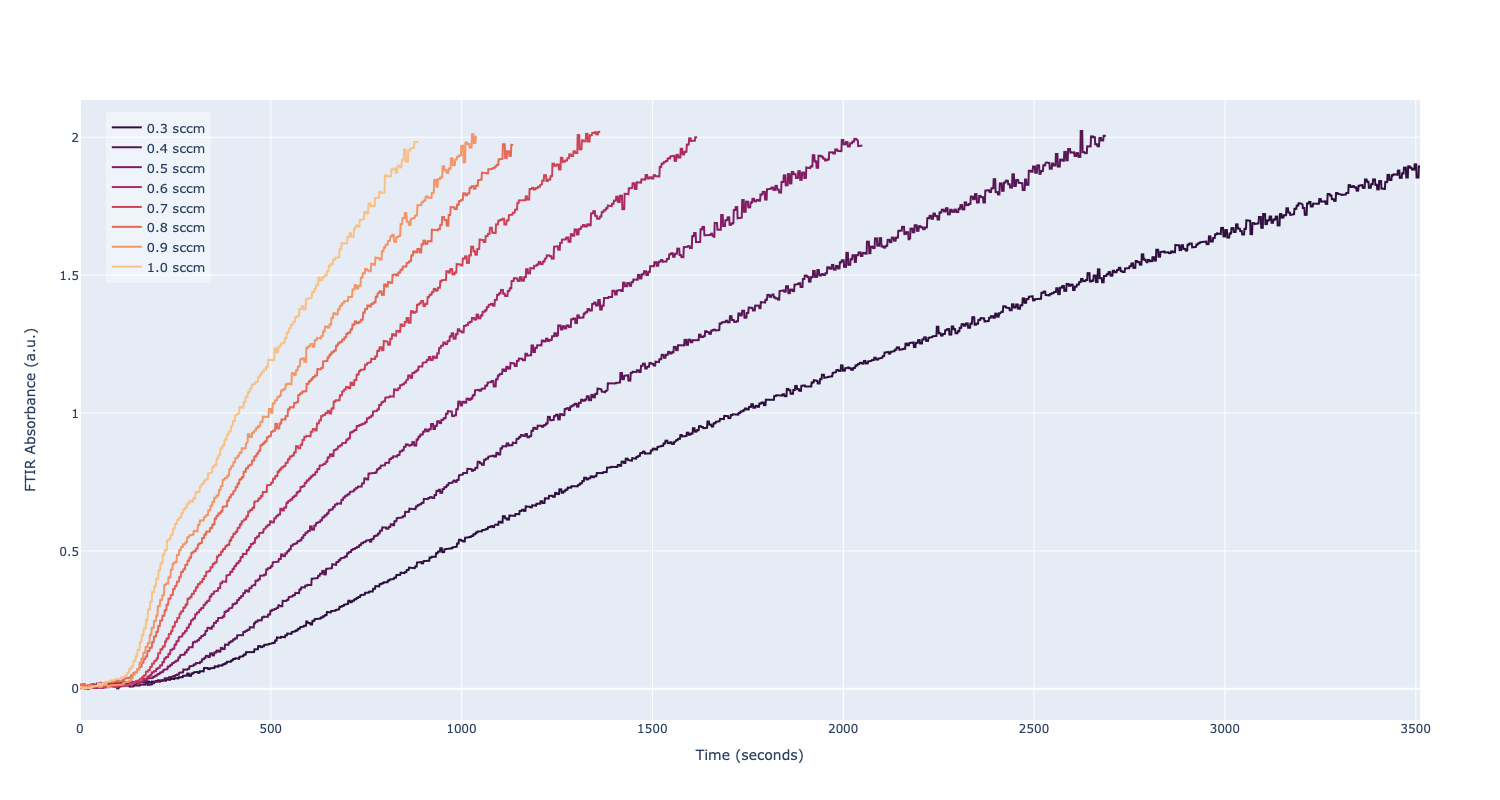
\includegraphics[width=\linewidth]{chapter_5/figures/CO2_gas_characteristation_raw.png}
	\caption{Time series response of the system without a CO$_2$ controller various flow rates of CO$_2$ gas.}
	\label{fig:CO2_gas_characteristation_raw}
\end{figure}

The raw results of this test can be seen in figure \ref{fig:CO2_gas_characteristation_raw}. The origin time, $t=0$, was set from the moment MFC$_4$ was turned on to let CO$_2$ into the system. CO$_2$ was only added until the FTIR read an absorbance of 2.0, which approximately equate to a 7\% CO$_2$-inert gas composition. The rationale for this is that values above this were too close to the limit of the CO$_2$ sample capabilities of the FTIR, meaning that any results would be very sensitive to noise.

The results shown mostly match the expected behaviour, wherein there is a (relatively) short lag time where the CO$_2$ concentration remains at 0 before the FTIR signal increases. However from the figure, it can be observed that there are some non-linear behaviour in the initial part the system response before linearising. Possible mechanisms for this are explained later, however for now there are two important characteristics to look at from this data. 

The first is the effect of CO$_2$ flow rate on the lag time of the system. This can be achieved by finding the inflection point of the curves, which simply involves finding the second derivative. However before this can be done, the data needs to be smoothed since derivatives are incredibly sensitive to noise. To achieve this, a gaussian filter was applied before each derivative was taken. An example of this process can be visualised in figure \ref{fig:inflection_point_process}. 

\begin{figure}[h!]
	\centering
	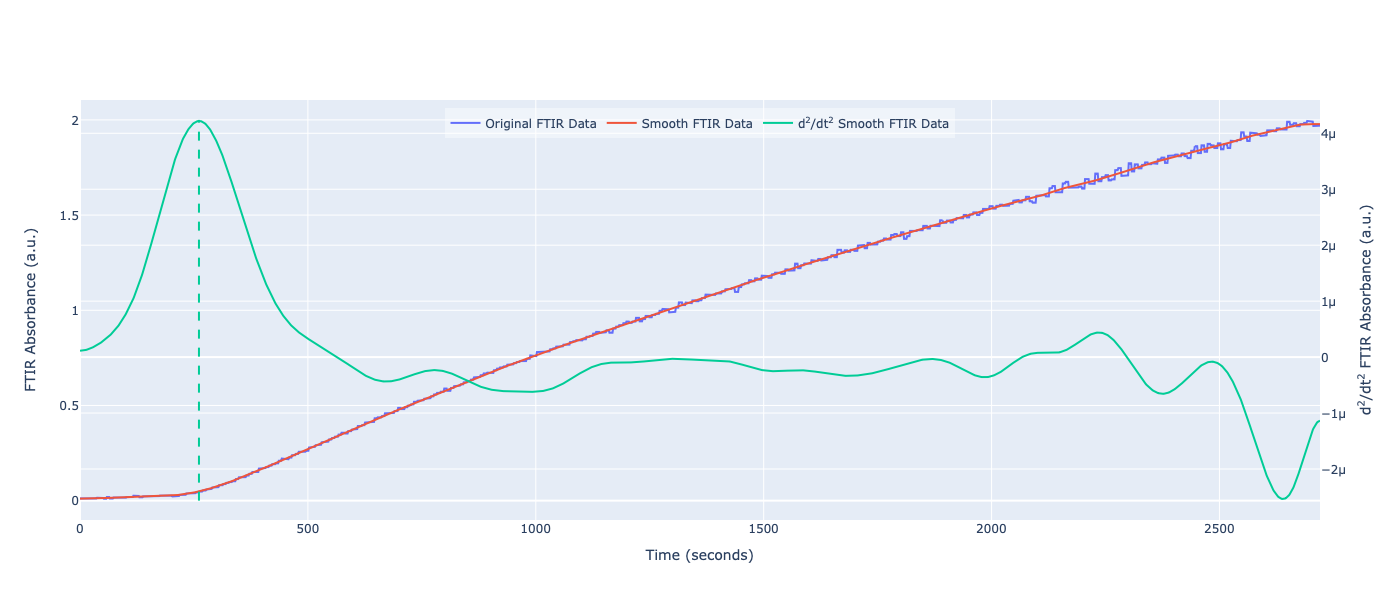
\includegraphics[width=\linewidth]{chapter_5/figures/inflection_point_process.png}
	\caption{Illustration of process used to determine the lag time of the system.}
	\label{fig:inflection_point_process}
\end{figure}

The results of this analysis can be seen in table \ref{tb:inflection_time_measured}. The inflection times measured have to be inversely proportional to the flow rate. This is because, as shown in equation \ref{eq:volumetric_flow_rate}, the flow rate is governed by the cross sectional area of the tube ($A$) and the velocity of gas going through it ($\nu$). Since the length of the tubing is fixed, the flow rate can be said to be:

\begin{equation}
    Q = V_{tube} \frac{1}{t}
\end{equation}
where $V_{tube}$ is simply the fixed volume of the tube.

\begin{table}[h!]
\centering
\caption{Measured lag time across various flow rates of CO$_2$ gas.}
\label{tb:inflection_time_measured}
\begin{tabular}{lr}
CO$_2$ flow rate (sccm) & Lag time (s) \\
0.3                  & 343.889             \\
0.4                  & 290.050             \\
0.5                  & 263.828             \\
0.6                  & 230.379             \\
0.7                  & 205.384             \\
0.8                  & 179.995             \\
0.9                  & 165.620             \\
1.0                  & 149.341            
\end{tabular}            
\end{table}

Using linear regression, a line of best fit can be obtained. This is shown in figure \ref{fig:inflection_times_best_fit}. The coefficients from the linear regression will be used in the Simulink model shown later.

\begin{figure}[h!]
	\centering
	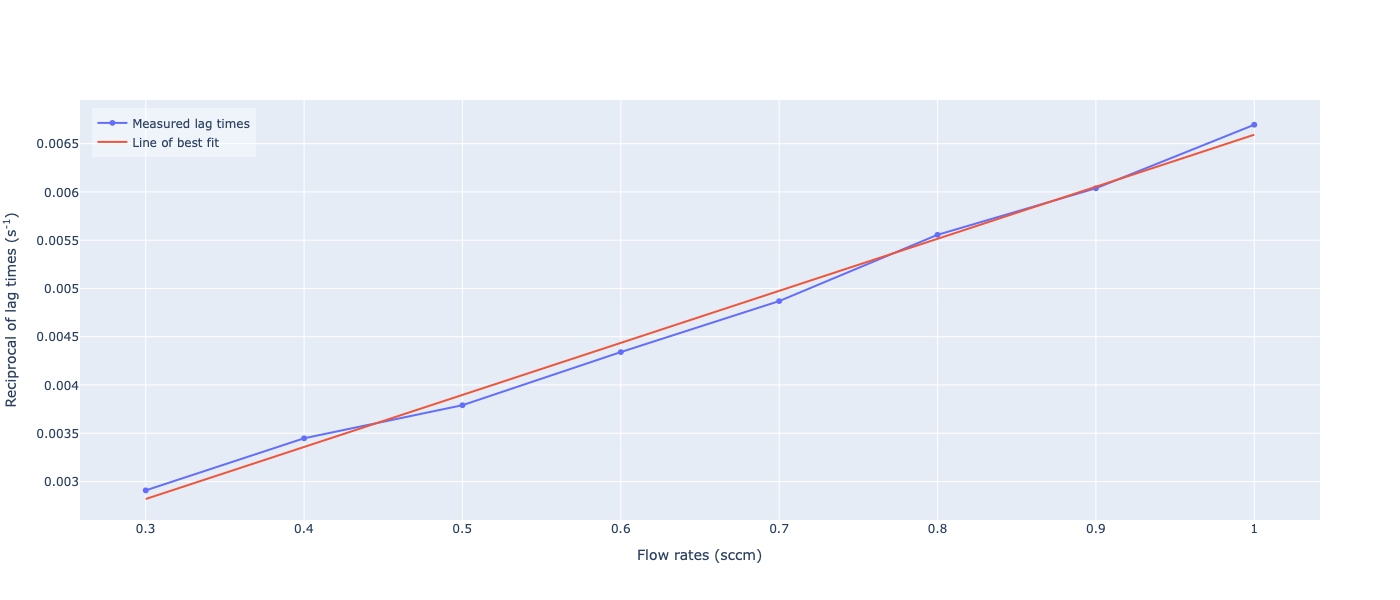
\includegraphics[width=\linewidth]{chapter_5/figures/inflection_times_best_fit.png}
	\caption{The inversely proportional relationship between flow rate and lag time.}
	\label{fig:inflection_times_best_fit}
\end{figure}

With the CO$_2$ lag times of the system characterised, the other characteristic to be determined is how the rate of CO$_2$ concentration increases with respect to the flow rate. As states previously, there appears to some non-linear behaviour in the system when the CO$_2$ concentration first increases. Hence, this characterisation process will only look at the results for when the FTIR absorbance is between 1.0-2.0. 

The expectation here is that the rate of increase of CO$_2$ concentration should be linear. The reason for this is that MFC$_4$ feeds a fixed volume of gas into the system, and since its pure CO$_2$ gas, the number of CO$_2$ molecules should entering the system at any given moment should be constant. Thus, since the system is a closed gas loop, the accumulation of CO$_2$ molecules should increase at a linear rate.

To achieve this, a slightly process was taken that in $\S$ \ref{subsec:pressure_in_srr_chamber} where the relationship between flow rate and the rate of increase in pressure were determined. This is because the FTIR data is inherently more noisy than the pressure readings. As such, rather than taking the gradient directly, a linear regression was first performed then the gradient of that line of best fit was used. An illustration of this process can be seen in figure \ref{fig:co2_characterisation_rate_of_increase_linearised}. Note that the origin times were reset so that $t = 0$ occurs when the FTIR absorbance first crosses 1.0.

\begin{figure}[h!]
	\centering
	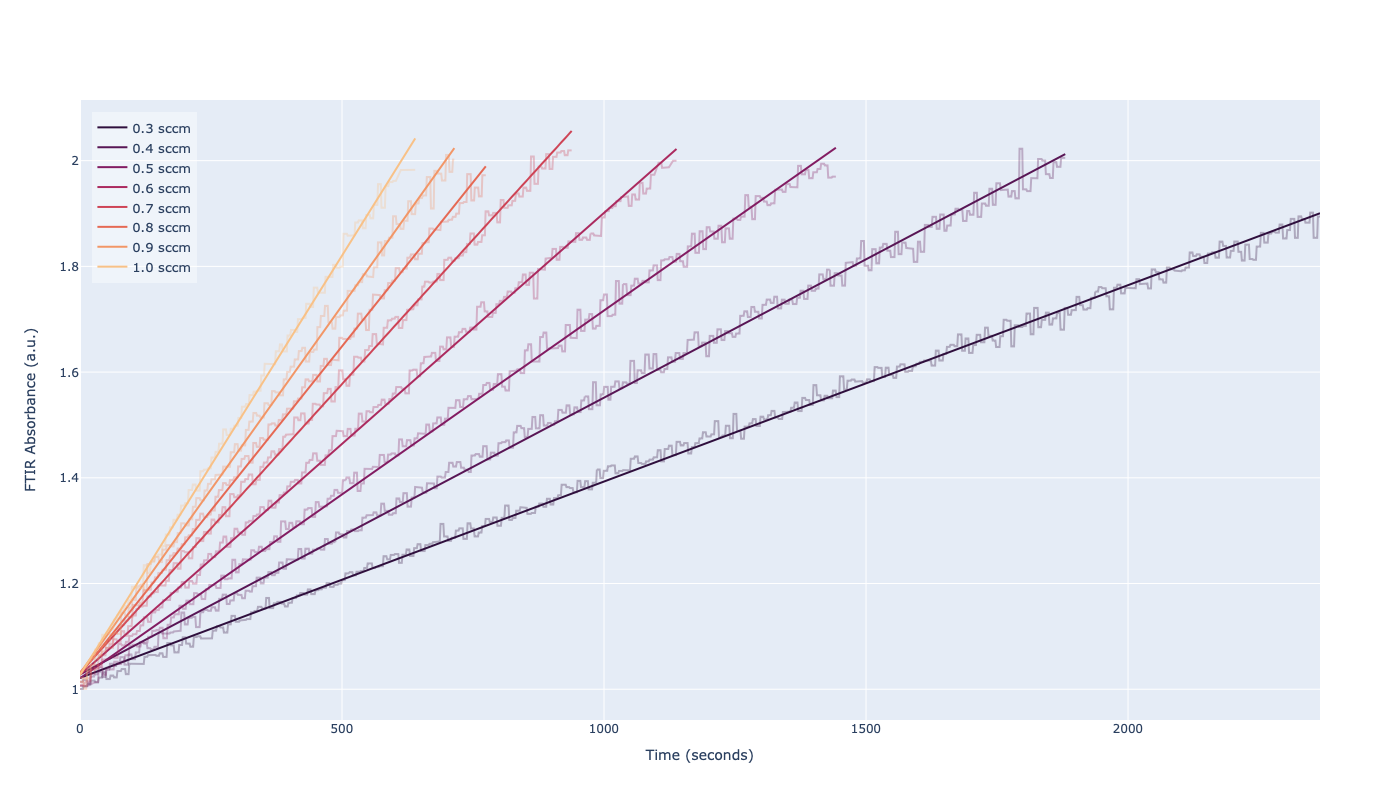
\includegraphics[width=\linewidth]{chapter_5/figures/co2_characterisation_rate_of_increase_linearised.png}
	\caption{Rate of change of CO$_2$ concentration for CO$_2$ flow rates between 0.3-1.0 sccm..}
	\label{fig:co2_characterisation_rate_of_increase_linearised}
\end{figure}

The gradient of the rate of change of CO$_2$ concentrations are shown in table \ref{tb:rate_of_change_absorbance_across_flow_rates_best_fit}, along with the corresponding coefficient of determination ($R^2$) values which denote the fit of the regression lines to the original data. All models have a $R^2 > 0.99$ with the worst values being 0.997, confirming the expected linear characteristic. 

\begin{table}[h!]
\centering
\caption{Best fit rate of change of FTIR absorbance across various flow rates.}
\label{tb:rate_of_change_absorbance_across_flow_rates_best_fit}
\begin{tabular}{ccr}
Flow rates (sccm) & Rate of change of FTIR absorbance (a.u.) & R2 Score \\
0.3               & 0.00037                                  & 0.99731  \\
0.4               & 0.00052                                  & 0.99672  \\
0.5               & 0.00070                                  & 0.99678  \\
0.6               & 0.00087                                  & 0.99721  \\
0.7               & 0.00109                                  & 0.99734  \\
0.8               & 0.00124                                  & 0.99760  \\
0.9               & 0.00139                                  & 0.99653  \\
1.0               & 0.00159                                  & 0.99754 
\end{tabular}
\end{table}

With the gradients determined, the relationship between those values and the flow rates can be visualised in figure \ref{fig:rate_of_change_of_absorbance_across_flow_rates}. The slope of the line will again be used in the Simulink model for the CO$_2$ controller.

\begin{figure}[h!]
	\centering
	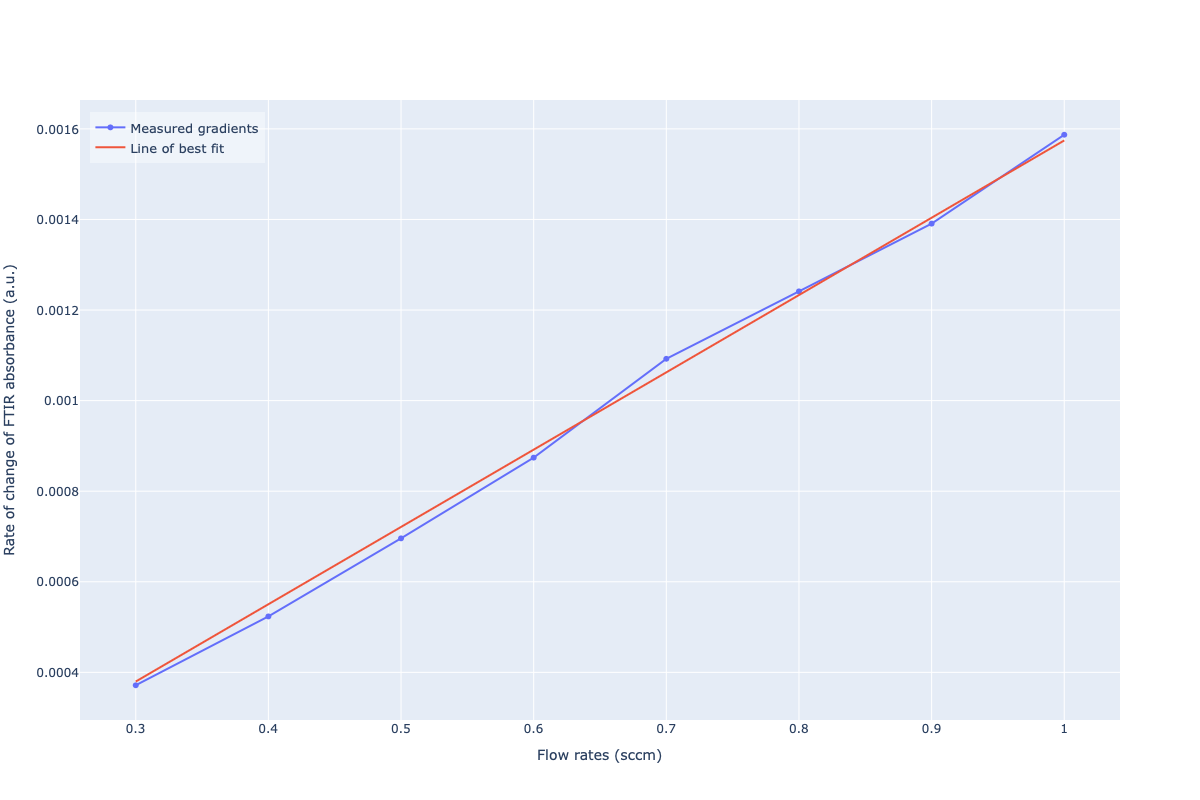
\includegraphics[width=\linewidth]{chapter_5/figures/rate_of_change_of_absorbance_across_flow_rates.png}
	\caption{Rate of change of CO$_2$ concentration for CO$_2$ flow rates between 0.3-1.0 sccm..}
	\label{fig:rate_of_change_of_absorbance_across_flow_rates}
\end{figure}

With these lag time and rate of change of CO$_2$ concentration characteristics obtained for various flow rates, the next step is to take these parameters into Simulink for modelling. The modelled control system can be seen in figure \ref{fig:p_controller_co2}. This is simply the ideal plant model (without incorporating errors from the mass flow controllers or the FTIR). 

\begin{figure}[h!]
	\centering
	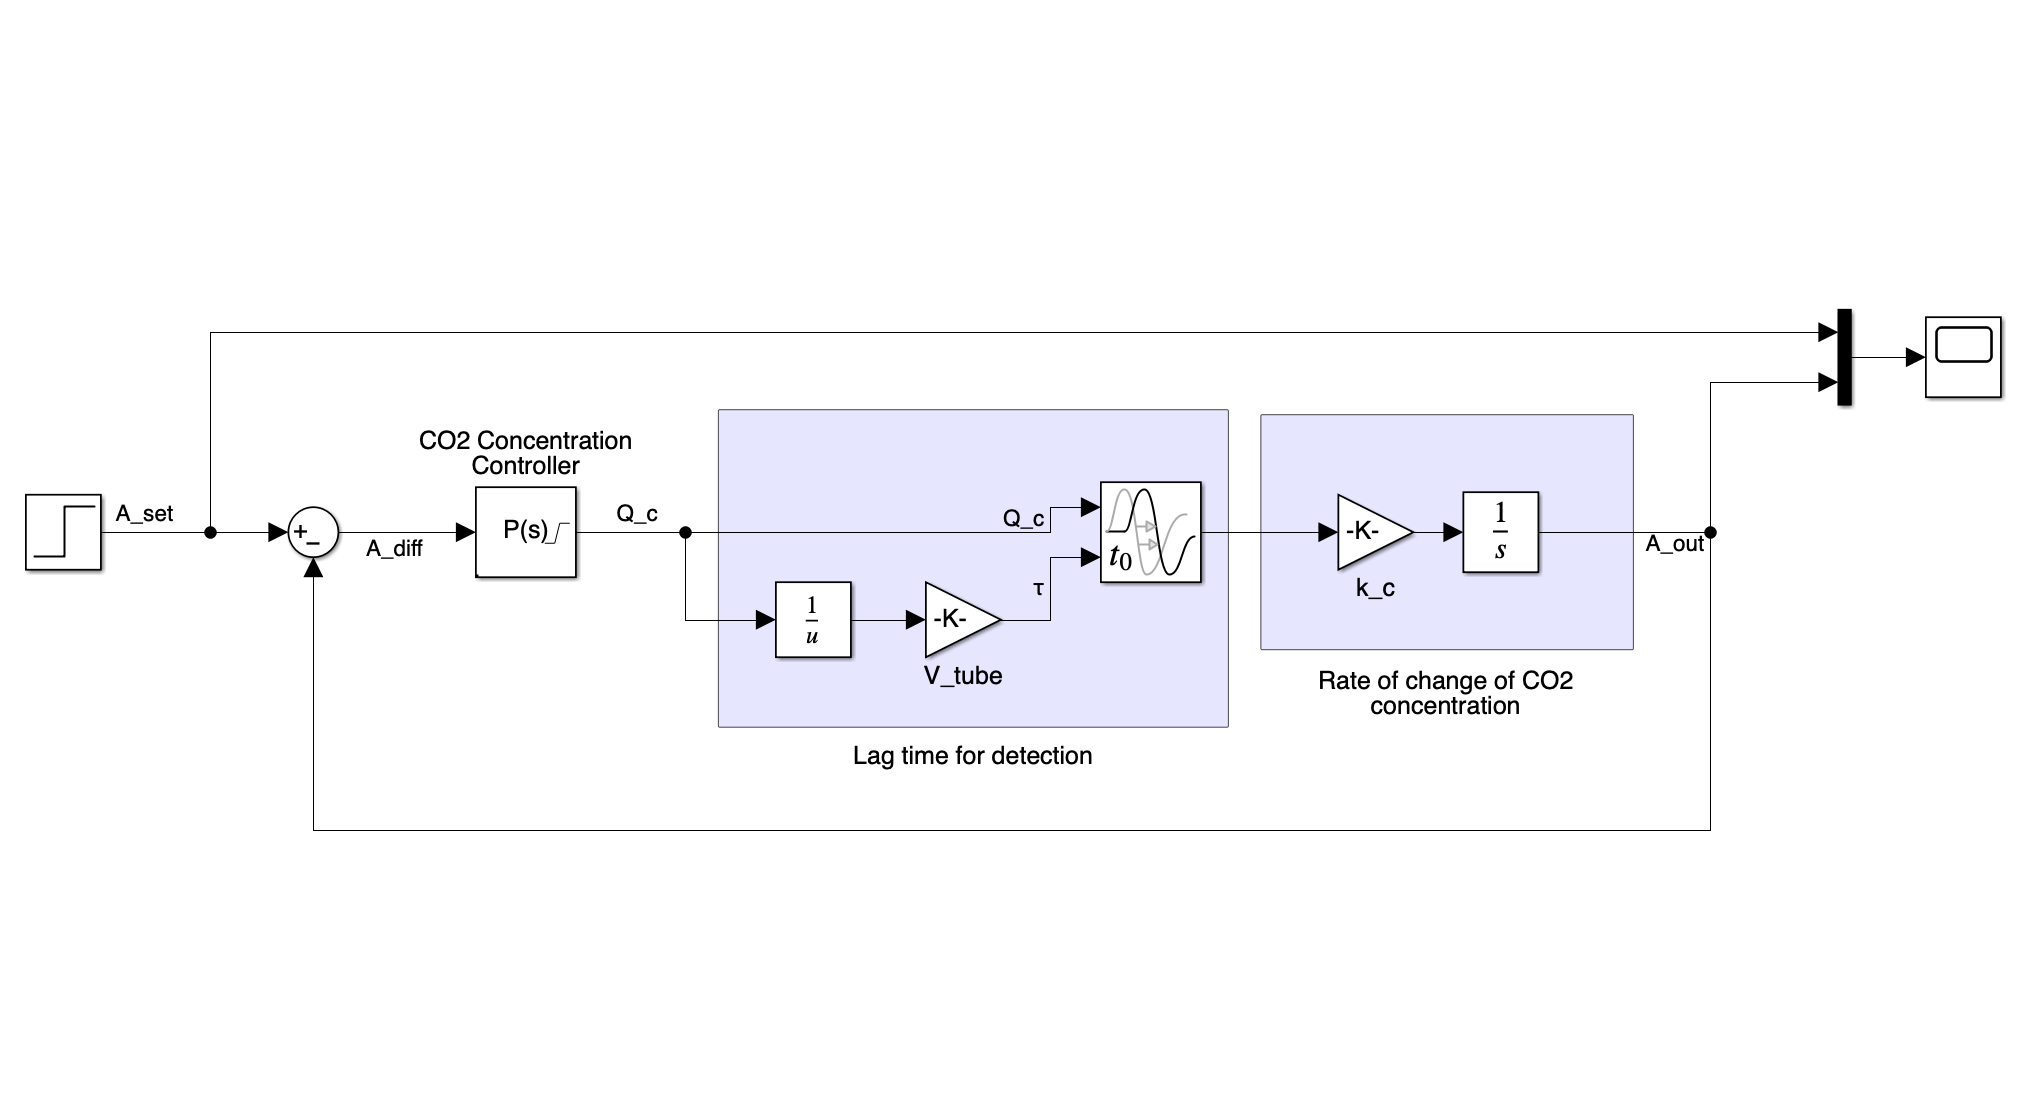
\includegraphics[width=\linewidth]{chapter_5/figures/ideal_p_controller_co2.png}
	\caption{Modelled CO$_2$ gas control system in Simulink.}
	\label{fig:ideal_p_controller_co2}
\end{figure}

The lag time is modelled using a variable time delay, based on the set CO$_2$ flow rate ($Q_{c}$) and the volume of the tubing ($V_{tube}$). It is governed by the equation:

\begin{equation}
    \tau = \frac{V_{tube}}{Q_{c}}
\end{equation}

As for the rate of change of CO$_2$ concentration, it is modelled identically to equation \ref{eq:transfer_function} in $\S$ \ref{subsec:pressure_in_srr_chamber}. The transfer function for the CO$_2$ plant is:

\begin{equation}
    A(s) = \frac{k_c}{s} Q_{c}(s)
    \label{eq:transfer_function_co2}
\end{equation}

where $A$ is the CO$_2$ absorbance measured by the FTIR and $k_c$ is the linear coefficient for the rate of change of CO$_2$ concentration; which was $k_c = 0.00171$.

A comparison between this ideal plant model to the results previously gathered for the CO$_2$ characterisations are shown in figure \ref{fig:real_vs_modelled_data}, specifically the the case with the flow rate $Q_c = 0.5$ sccm. At a glance, it is very obvious that the real world data and the model do not match. However, it appears that bulk of this error between to two graphs occurs during the initial phase of the CO$_2$ concentration increasing. Then after some time the error plateaus, as the two graphs rise in parallel. 

\begin{figure}[h!]
	\centering
	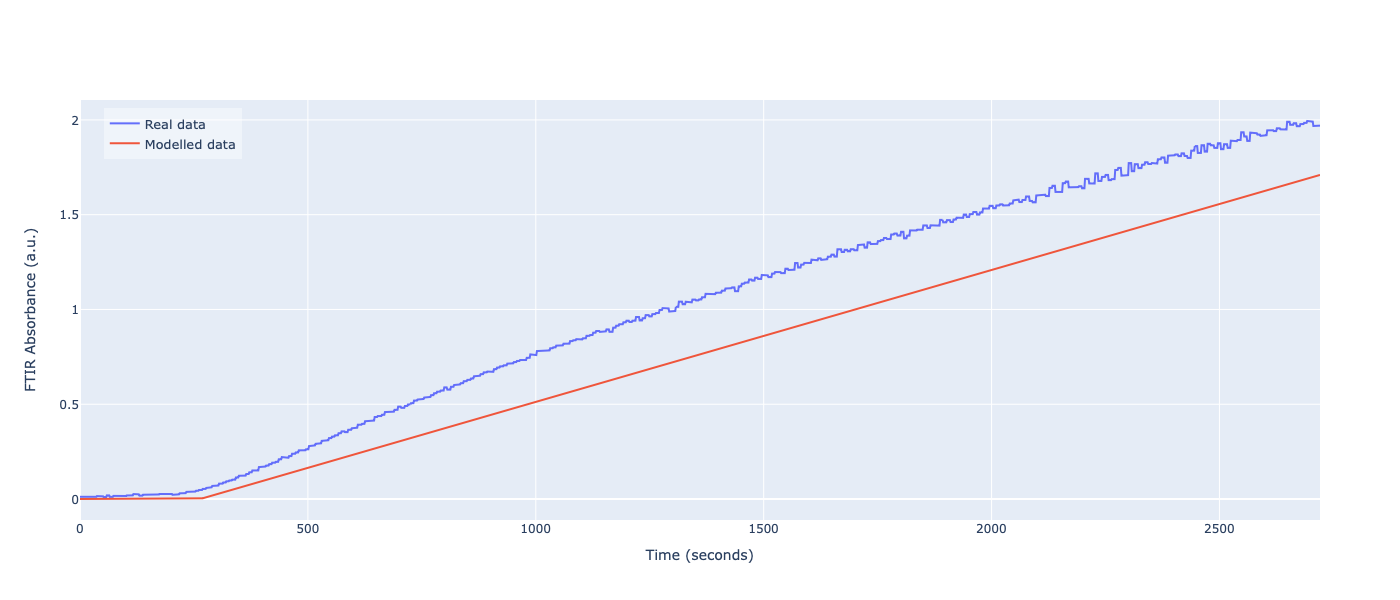
\includegraphics[width=\linewidth]{chapter_5/figures/real_vs_modelled_data.png}
	\caption{Comparison between the (real) measured characterisation data and modelled data for the flow rate $Q_c = 0.5$ sccm.}
	\label{fig:real_vs_modelled_data}
\end{figure}

This behaviour is confirmed for all flow rates by taking the difference between the real and modelled data, shown in figure \ref{fig:difference_between_real_vs_modelled_data}. There could potentially be several reasons for this error in the initial phase, though the most likely reason is probably due to the mixing of the inert gases and CO$_2$. This explains why after a period of time this error plateaus as the gas mixture is fully homogenous.

\begin{figure}[h!]
	\centering
	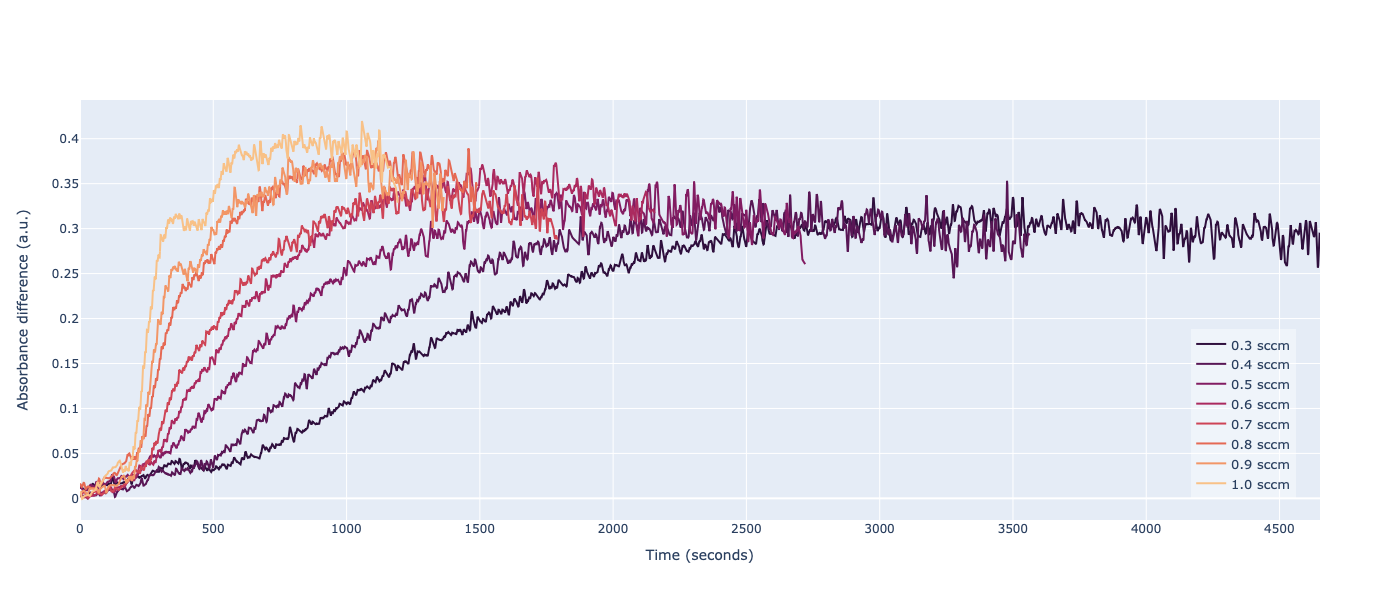
\includegraphics[width=\linewidth]{chapter_5/figures/difference_between_real_vs_modelled_data.png}
	\caption{Difference between real and modelled data for all flow rates tested.}
	\label{fig:difference_between_real_vs_modelled_data}
\end{figure}

The other difference in behaviour seen in figure \ref{fig:difference_between_real_vs_modelled_data} is that for the flow rates of 0.9 and 1.0 sccm, there are two plateaus; which implies that there is a separate mechanism occurring here. Indeed, if one refers back to figure \ref{fig:CO2_gas_characteristation_raw}, there appears to be a slight plateau before the FTIR signal continues to increase again. The most likely explanation here is that at higher   flow rates, the CO$_2$ concentration is saturated since there was not sufficient time for the CO$_2$ gas to complete the closed loop yet and begin accumulating in the system. To confirm this behaviour, additional tests were done with flow rates of 2.0 and 3.0 sccm of CO$_2$ gas, shown in figure \ref{fig:co2_system_characterised_large_flow_rates}. From the figure, the plateaus are even more prominent, confirming the hypothesis for this behaviour.

\begin{figure}[h!]
	\centering
	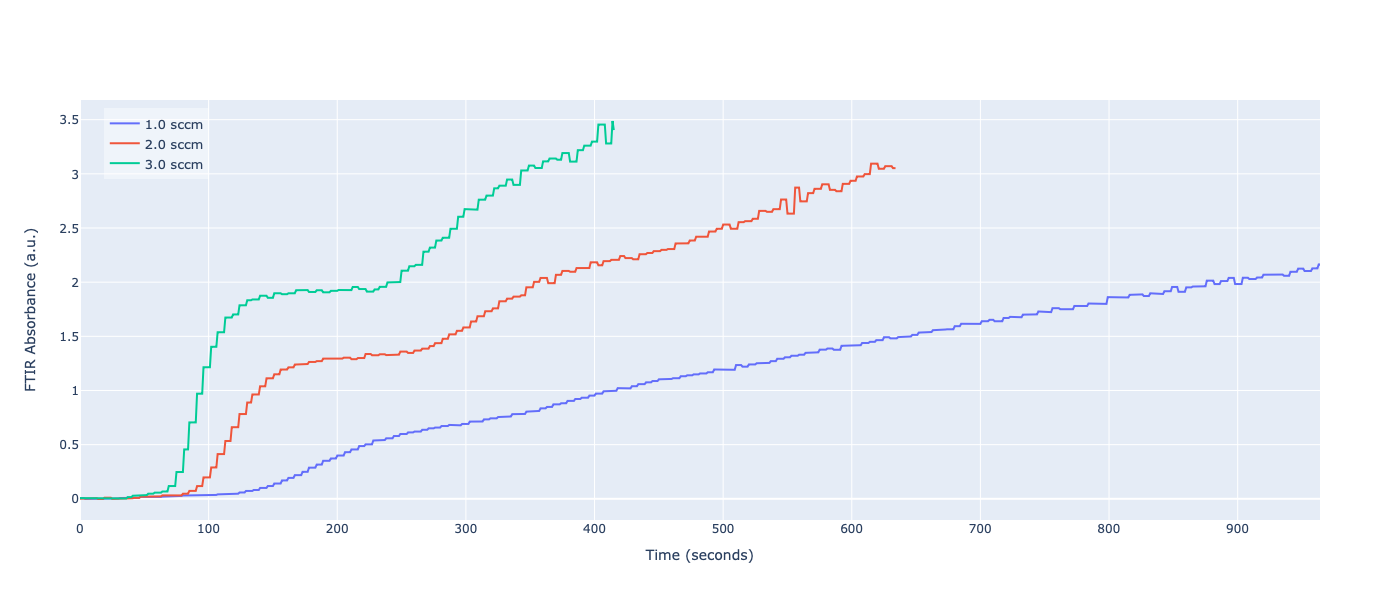
\includegraphics[width=\linewidth]{chapter_5/figures/co2_system_characterised_large_flow_rates.png}
	\caption{Time series response of system (without a CO$_2$ controller) for larger flow rates.}
	\label{fig:co2_system_characterised_large_flow_rates}
\end{figure}

Nevertheless, even though the model generated does not exactly match the real data, it is sufficient to understand the basic mechanics of the control system and give the author an idea of the type of controller to be used. As such, proportional only controller was chosen. This is because of the large lag time of the system would mean that if a PI controller were to be used, a large integration error would be present which would cause a large but temporary overshoot of the setpoint CO$_2$ concentration. This was not an issue with the Helium gas only controller since there was effectively no lag in the system, meaning there was minimal overshoot thus no effect on the plasma. However, a large overshoot in the CO$_2$ composition of the plasma would result in an increase in the deposition of carbon on the SRR gap itself. This would either extinguish the plasma, or worse block the orifices for the gas to flow through. 

A proportional only controller would eliminate this issue, though this comes at the cost of time performance and potentially an offset error. The former is an inconvenience, but seeing as the system is a proof of concept, it is not necessarily a deal-breaker. The offset error would be more of an issue, but this again depends on the severity of the error. The only way to determine this was run the model and evaluate how it performed.

For the proportional controller, a unity gain was set. Setting the gain higher would in theory improve the time taken for the system to reach steady state. However as stated earlier, with the higher flow rates, there is not a sufficient amount of time for the CO$_2$ gas gas to complete the closed loop. This could lead to overshoots if the CO$_2$ concentrations were set to lower values. With this, a comparison of the modelled performance and the real-world performance of this controller was done. The controller was instructed to reach a FTIR absorbance set point of 0.3, which is approximately equivalent to a 1\% CO$_2$ gas mixture.


\begin{figure}[h!]
	\centering
%	\includegraphics[width=0.8\linewidth]{example-image-a} 
    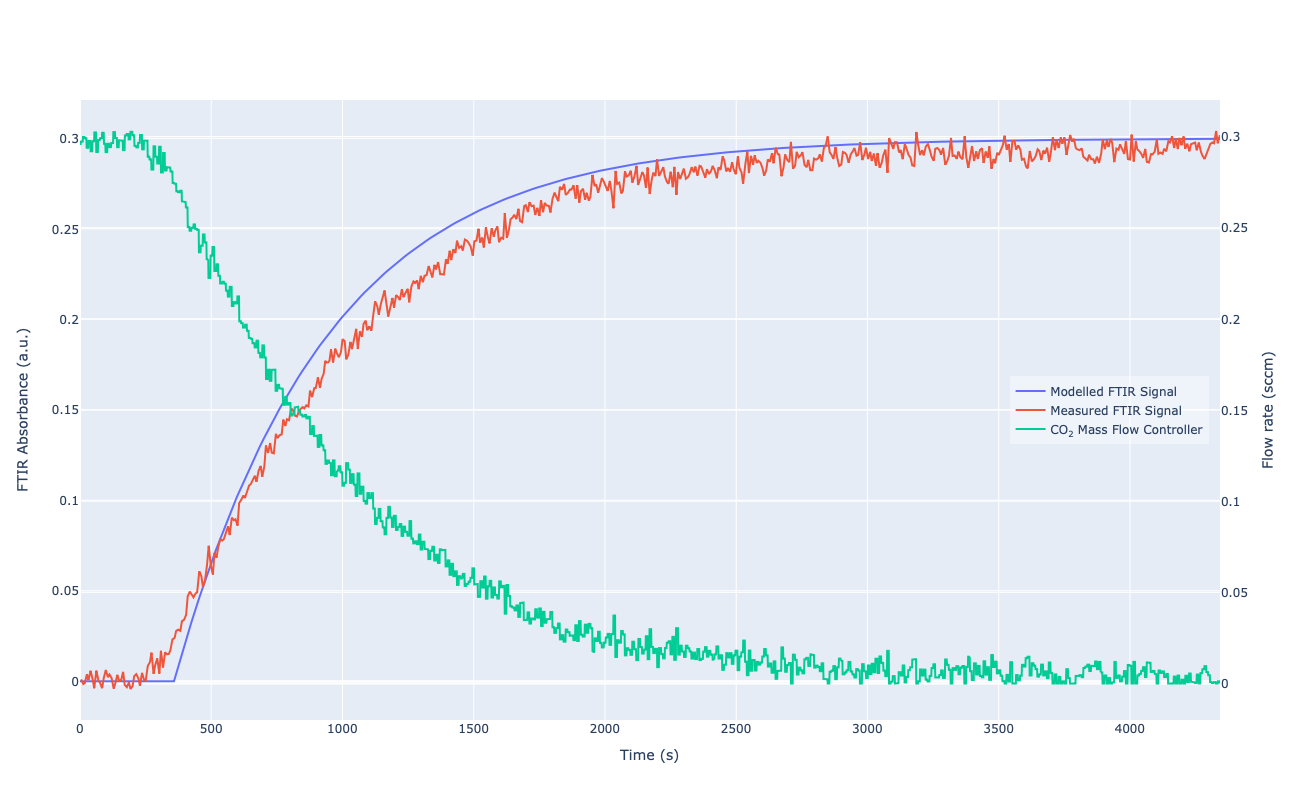
\includegraphics[width=\linewidth]{chapter_5/figures/model_vs_real_co2_controller.png} 
	\caption{Comparison between the modelled and real proportional controllers for regulating CO$_2$ concentrations.}
	\label{fig:model_vs_real_co2_controller}
\end{figure} 

Figure \ref{fig:model_vs_real_co2_controller} shows the results of this comparison.
From the data, it can be seen that the modelled performance quite closely matched the measured results. The measured lag time in this test appears to be slightly shorter, but is still in line with the results seen in table \ref{tb:inflection_time_measured}. 

As for the rise of the FTIR absorbance, the real world results seems to indicate a slower rise compared to the model. Though this is explained by the fact that at flow rates below 0.3 sccm, the mass flow controller struggles to continuously output a fixed flow rate, instead relying on PWM. This is more evident when measuring the settling time. In the previous section on the pressure controller, the settling time was measured in terms of 0.1\% of the set point. However, due to the relatively small values of the FTIR absorbance, the settling time taken was to 5\% of the set point (in this case, an absorbance of 0.29). 

The settling time for model was approximately 2300 seconds ($\approx 38$ minutes) whereas the settling time for the real world controller was around 2800 seconds ($\approx 46$ minutes). These are relatively large wait times, especially when compared to the pressure controller results. However, since the system is designed to intended to be run continuously for several hours at a time, such wait times the start of the process were deemed to be acceptable.


%Nonetheless, the equation in \ref{eq:linearised_conc_moles} determines the concentration using moles of gas, but the input into the control system will be a given flow rate of CO$_2$. While this conversion can be determined analytically, since it is essentially a conversion between molar flow rate to volumetric flow rate, the fact that the gas is being compressed in the system within the secondary chamber adds some complexity to this. As such, it would be easier to determine this relationship experimentally.

%To achieve this, the change of CO$_2$ concentration with respect to time was measured by the FTIR across several flow rates of CO$_2$, between 0.5 to 1.0 sccm. The system was set up in a way such that the Helium control system would pressurise the system as normal. Then once system was in equilibrium, MFC$_4$ was set to a fixed flow rate, which controls the amount of CO$_2$ entering the system. Once MFC$_4$ is set, the total pressure of the overall system increases so the ``topping up'' of Helium gas by the controller ceases. The results of this experiment can be seen in figure \ref{}.

%From the results, it can be seen that the delay of detecting CO$_2$ gas was again present (as noted earlier in this subsection), though the time of the delay is dependant on the flow rate of CO$_2$. This makes intuitive sense, as increasing the flow rate also increases the average velocity of gas, which in turn reduces lag time of detection. From the figure, it can also be seen that the rate of change of CO$_2$ concentration increases somewhat linearly. The average slope for this can be seen in table \ref{}.






\subsection{Carbon monoxide concentrations}

With the CO$_2$ controller functioning with the presence of the plasma, an interesting observation can be seen in the FTIR spectra. In addition to the CO$_2$ peaks (and the peaks due to presence of water vapour), there are strong peaks of CO present in the system. This was also observed in the open gas loop configuration with the FTIR placed after the plasma, but this signal was quite weak due to the fact that only a small amount of CO as formed and all the gas was vented to atmosphere. With the closed gas loop configuration, since the gas is recycled, its concentration can build up resulting in more visible peaks. 

For the purposes of this report, the CO concentration will not be quantified simply because of the lack of access to pure CO to produce a calibration curve (like that performed on CO$_2$). However, this system could be easily adapted to control the concentration CO instead of CO$_2$ if needed. Nevertheless, the accumulation of CO in the system adds further proof that the CO$_2$ is being dissociated, meaning that the epoxidation process will occur.

\begin{figure}[h!]
	\centering
	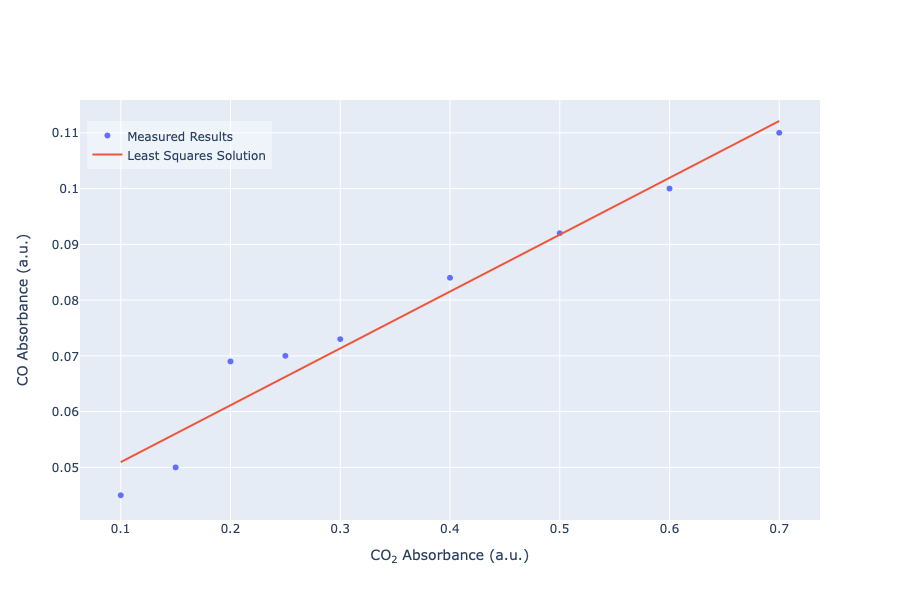
\includegraphics[width=\linewidth]{chapter_5/figures/co2_vs_co_absorbance.png} 
	\caption{Comparison CO$_2$ and CO absorption in the FTIR spectra.}
	\label{fig:co2_vs_co_absorbance}
\end{figure} 

One observation seen with the CO results in the FTIR is that the absorption peaks settle to fixed value after a period of time. This is to be expected since the CO$_2$ dissociation reaction is reversible, thus it should settle into a steady state after some time. Since every molecule of CO$_2$ should produce one molecule of CO, one should expect a linear relationship between the absorption of both these molecules. 

To asses this, the CO$_2$ controller was used to set CO$_2$ concentration set points between 0.5\% to 3\%, and the steady state CO absorptions were measured. The results of this test can be seen in figure \ref{fig:co2_vs_co_absorbance}.

 \begin{figure}[h!]
	\centering
	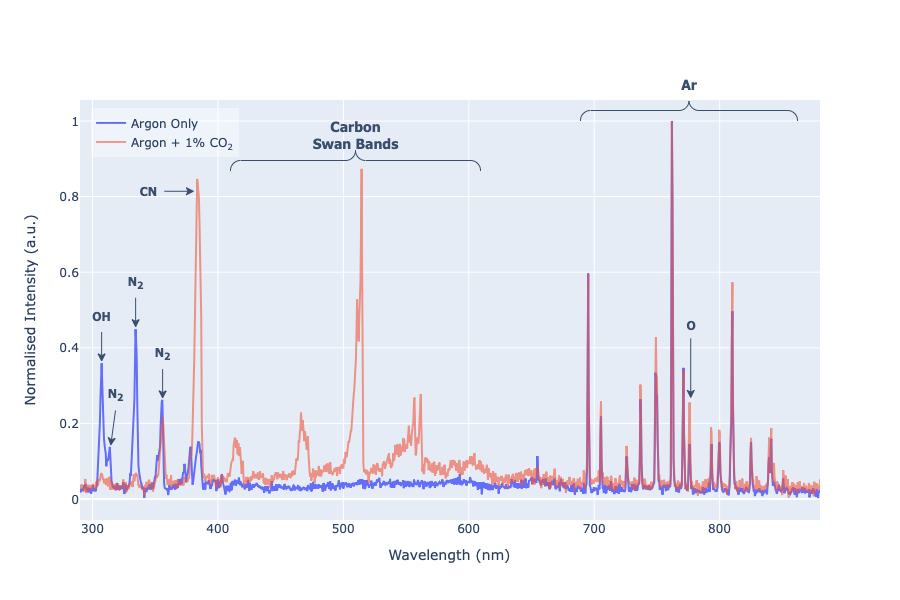
\includegraphics[width=0.95\linewidth]{chapter_5/figures/optica_spectra_co2.png} 
	\caption{Optical spectra between pure Argon plasma and Argon plasma with CO$_2$.}
	\label{fig:optica_spectra_co2}
\end{figure} 

 From the results, a linear relationship was observed though the relationship was not proportional. This is most likely due to the fact that the system does contain some nitrogen gas impurities, which could be reacting with the atomic oxygen producing nitrogen oxides (NO and NO$_2$), or reacting with the carbon to produce cyanide (CN). Additionally, the carbon deposition on the SRR may play a role in the loses. In the optical spectra, the nitrogen oxides peaks are not particular visible because they tend to be quite broad. However, the CN peak is strongly visible and also the carbon peaks from the Swann bands. This can be seen in figure \ref{fig:optica_spectra_co2}. (Note that test was done using an Argon plasma instead of a Helium plasma, but the results should be the same.)
 




%\pagebreak 

\section{Overall Control System performance}


With the two parts of the control system functioning as expected when compared to the Simulink models, the next step was to evaluate the long-term performance of the system. This is because the goal is to run this experimental setup for hours at a time, and potentially even days. While there weren't any issues in the short-term tests when correlating with the models, there could potentially be issues when running for longer periods of time. As such, the control system  was left to run over the period of 24 hours. The result of this can be seen in figure \ref{fig:24_hour_test_run}.

\begin{figure}[h!]
	\centering
	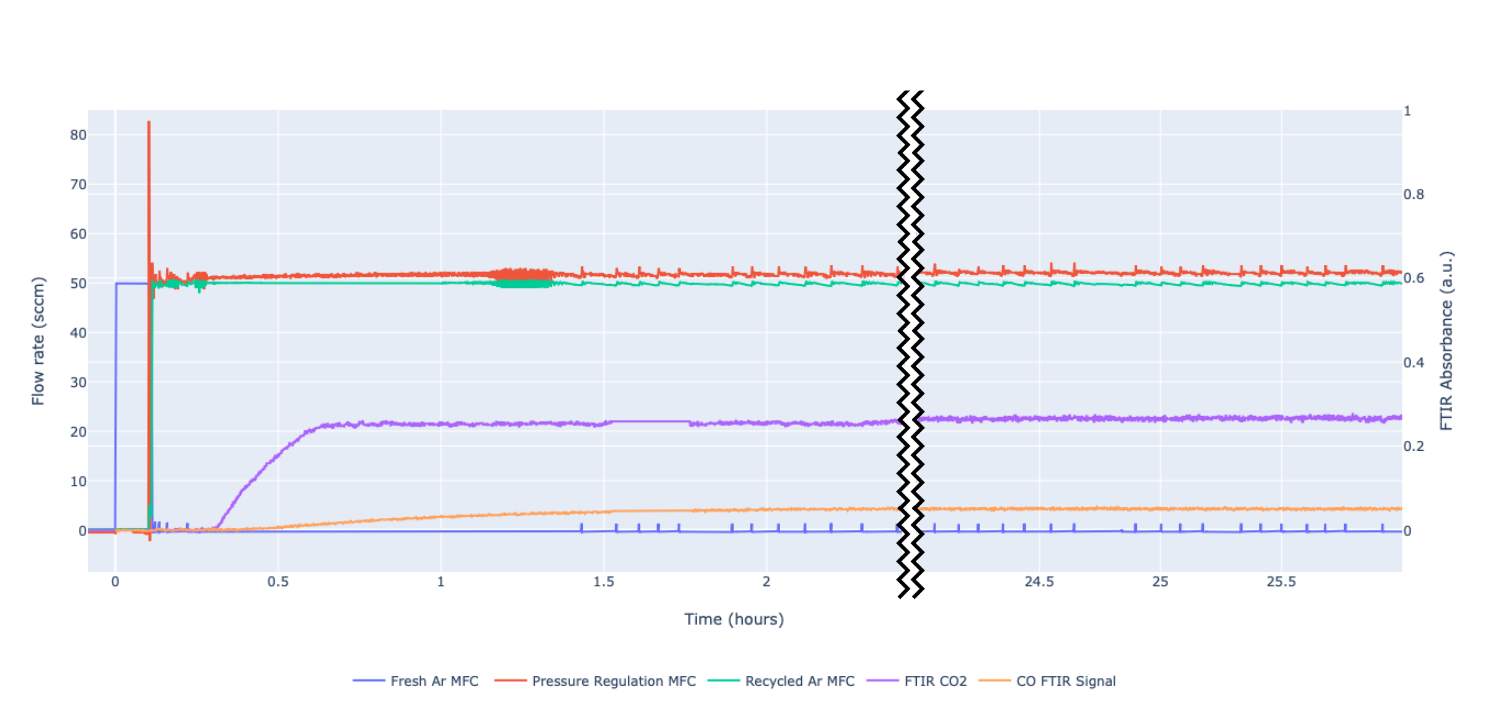
\includegraphics[width=\linewidth]{chapter_5/figures/24_hour_test_run.png}
	\caption{Time series plot of the mass flow controller and FTIR traces of the control system operating over a 24 hours.}
	\label{fig:24_hour_test_run}
\end{figure}

The test used the typical set points for the control system, which were a main chamber pressure of 760 Torr,  a secondary chamber pressure of 910 Torr, and a CO$_2$ gas concentration of 1\%. While figure \ref{fig:24_hour_test_run} does not show the time series traces from both pressure sensors, both values were kept relatively constant once the system was in steady state. Additionally, figure \ref{fig:24_hour_test_run} does not show the mass flow controller response of MFC$_4$ (for the CO$_2$ gas input) because the traces were not visible due to the scale of the response; the maximum mass flow reading was 0.3 sccm of CO$_2$ gas. 

The short-term performance (i.e. the first hour) of the system was inline with previous results. Between the period of 70-80 mins, there was a slight abnormality in the in the MFC$_2$ and MFC$_3$ response whereby the signal was quite noisy; though this returned back to normal afterwards. After that, the control system began gradually ``topping-up'' the main chamber with some additional feed gas. There was another anomaly, this time in the FTIR signal between 90-105 minutes after starting the test, though this was because the FTIR stopped sampling data periodically and needed to be restarted. However, since the CO$_2$ concentration of the system was already saturated at 1\%, this did not cause any issue. Aside from that, no other issues occurred in the system.

Aside from those two minor issues, the long-term tests show that the system performed satisfactorily. The noble gas usage, once the system was in steady state, was a minimal. In the first 20 minutes of the system, when the system was first pressuring and left to equilibrate, the total Helium used was 335 cm$^3$. Then over the next 24 hours, the total fresh gas inputted into the system was only 15 cm$^3$, only 4\% of the gas used to originally fill up the system. This gave an equivalent flow rate of approximately 0.01 sccm of Helium gas once in the steady state, which is a 5000 times reduction in gas usage. 


In terms of characterisation of the ``topping-up'' mechanism, figure \ref{fig:top_up_characteristics} shows the histogram of the ``top-up'' interval and volume. 

\begin{figure}[h!]
    \centering
    \begin{subfigure}{0.8\linewidth}
        \centering
        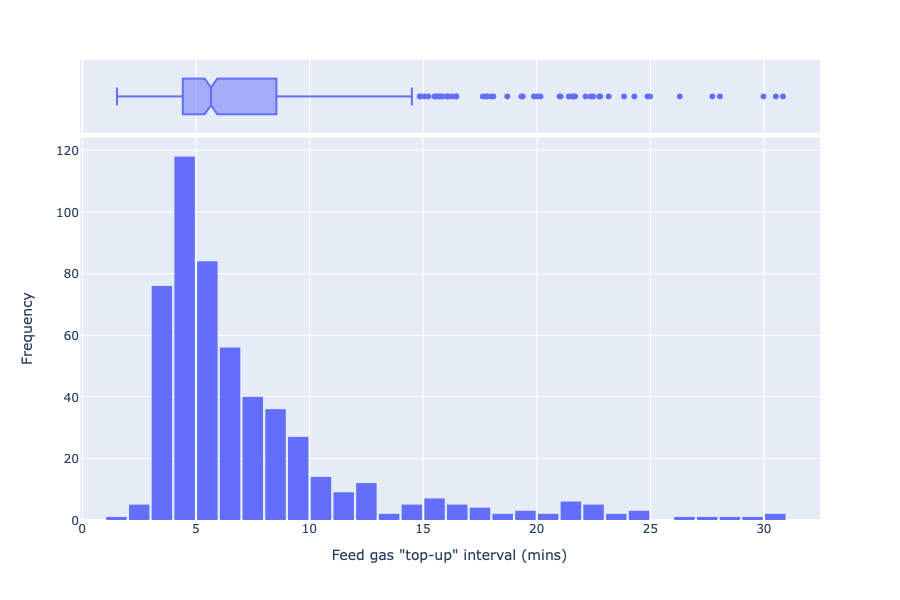
\includegraphics[width=\linewidth]{chapter_5/figures/top_up_interval.png}
        \caption{}
    \end{subfigure}
    \begin{subfigure}{0.8\linewidth}
        \centering
        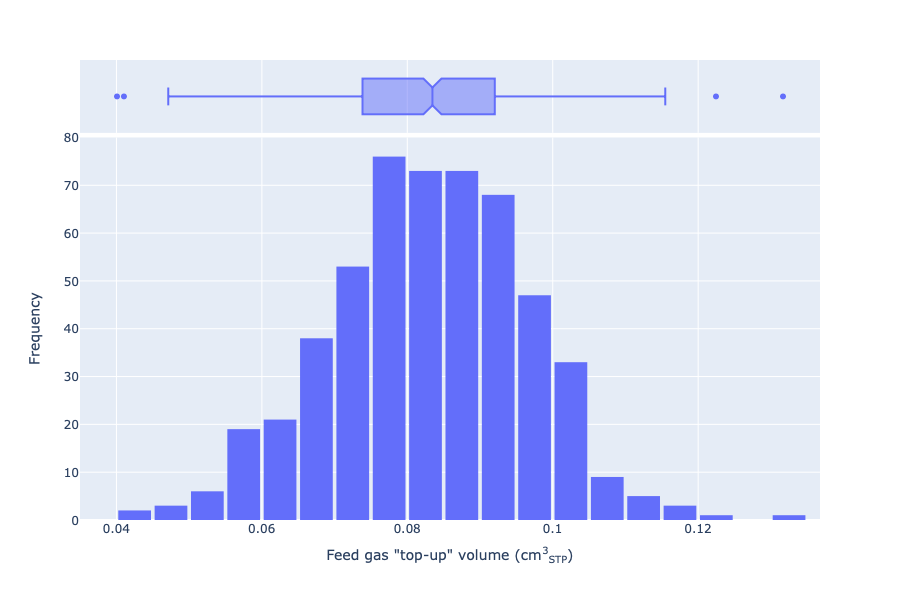
\includegraphics[width=\linewidth]{chapter_5/figures/top_up_volume.png}
        \caption{}
    \end{subfigure}
    \caption{``Top-up'' interval (a) and gas volume (b) of the system.}
    \label{fig:top_up_characteristics}
\end{figure}

The median ``top-up'' interval of the system was 5.6 minutes, with the mode being between 4-5 minutes and results longer than 15 minutes being outliers. While an ideal system would not require any refilling of the system, this performance is satisfactory. In terms of the ``top-up'' volume, this was more inline with a normal distribution with the mean (and median) volume being 0.083 cm$^3$.









%
%
%As stated previously, when the SRR was running with a helium and CO$_2$ plasma in an open gas loop configuration, the concentration of CO$_2$ ($c$) was determined using the 
%Though not directly applicable for running the plasma in a closed gas loop configuration, the general principle of this expression can be used. This is because  
%
%
%Since the flow rate is governed as the rate of change of the number of moles for a given cross sectional area ($Q = \frac{\partial n}{\partial t}$)
%
%
%In the closed gas loop system shown in figure \ref{fig:He_CO2_control_system}, gas can only enter the system via MFC$_1$ or MFC$_4$. As such, in an ideal system with no losses, the concentration of CO$_2$ can be expressed as:
%
%\begin{equation}
%    c = \frac{n_{CO_2}}{n_{He} + n_{CO_2}}
%\end{equation}
%


%
%- in open loop, the co2 conc is modelled exponentially
%- in closed loop, the co2 conc is modelled linearly, where the 





